 % use the "wcp" class option for workshop and conference
 % proceedings
 %\documentclass[gray]{jmlr} % test grayscale version
 %\documentclass[tablecaption=bottom]{jmlr}% journal article
 \documentclass[tablecaption=bottom,wcp]{jmlr} % W&CP article

 % The following packages will be automatically loaded:
 % amsmath, amssymb, natbib, graphicx, url, algorithm2e

 \usepackage{rotating}% for sideways figures and tables
 %\usepackage{longtable}% for long tables

 % The booktabs package is used by this sample document
 % (it provides \toprule, \midrule and \bottomrule).
 % Remove the next line if you don't require it.
\usepackage{booktabs}
 % The siunitx package is used by this sample document
 % to align numbers in a column by their decimal point.
 % Remove the next line if you don't require it.
\usepackage[load-configurations=version-1]{siunitx} % newer version
 %\usepackage{siunitx}
 \usepackage{booktabs}
\usepackage{amsmath}
\usepackage{enumitem}
\usepackage{algorithm}
% \bibliography{references}

\usepackage{comment}
\usepackage{multirow}
% operators

% \newcommand{\argmax}{\operatornamewithlimits{argmax}}
% \newcommand{\argmin}{\operatornamewithlimits{argmin}}

% vectors
\let\avec\vec
%\renewcommand{\vec}[1]{\ensuremath{\boldsymbol{#1}}}
\renewcommand{\v}[1]{\ensuremath{\boldsymbol{#1}}}

\newcommand{\src}{\lstinline[mathescape, keepspaces]}
\newcommand{\msrc}[1]{\mbox{\src!#1!}}

% \newcommand{\tens}[1]{%
%   \mathbin{\mathop{\otimes}\limits_{#1}}%
% }

% symbol shorthands (lowercase)
\newcommand{\vx}{\ensuremath{\v{x}}}
\newcommand{\vy}{\ensuremath{\v{y}}}
\newcommand{\vz}{\ensuremath{\v{z}}}
%\newcommand{\h}{\v{\eta}}
%\newcommand{\e}{\v{\epsilon}}
%\renewcommand{\u}{\v{u}}
\newcommand{\pd}{\ensuremath{\partial}}
\newcommand{\x}{\ensuremath{x}}
\newcommand{\y}{\ensuremath{y}}
\newcommand{\z}{\ensuremath{z}}
\newcommand{\h}{\ensuremath{\eta}}
\newcommand{\e}{\ensuremath{\epsilon}}
\renewcommand{\u}{\ensuremath{u}}
\newcommand{\q}{\theta}
\newcommand{\f}{\phi}
\renewcommand{\l}{\lambda}
\renewcommand{\t}{\tau}

% symbol shorthands (uppercase)
\renewcommand{\L}{\ensuremath{\mathcal{L}}}
% \newcommand{\KL}[2]{\ensuremath{\mathrm{KL}\left({#1} \:\middle\vert\middle\vert\: {#2}\right)}}
% \newcommand{\E}{\ensuremath{\mathbb{E}}}
\newcommand{\N}{\ensuremath{\mathcal{N}}}
\newcommand{\C}{\ensuremath{\mathtt{Concrete}}}

%\let\lmid\mid
%\renewcommand{\mid}{\!\lmid\!}

\newcommand{\eval}{\ensuremath{$\reflectbox{$\,\leadsto\,$}$}}
%\newcommand{\eval}{\sim}
\newcommand{\hide}[1]{}

\makeatletter
\DeclareRobustCommand{\cev}[1]{%
  \mathpalette\do@cev{#1}%
}
\newcommand{\do@cev}[2]{%
  \fix@cev{#1}{+}%
  \reflectbox{$\m@th#1\vec{\reflectbox{$\fix@cev{#1}{-}\m@th#1#2\fix@cev{#1}{+}$}}$}%
  \fix@cev{#1}{-}%
}
\newcommand{\fix@cev}[2]{%
  \ifx#1\displaystyle
    \mkern#23mu
  \else
    \ifx#1\textstyle
      \mkern#23mu
    \else
      \ifx#1\scriptstyle
        \mkern#22mu
      \else
        \mkern#22mu
      \fi
    \fi
  \fi
}


 % The following command is just for this sample document:
\newcommand{\cs}[1]{\texttt{\char`\\#1}}% remove this in your real article

 % Define an unnumbered theorem just for this sample document for
 % illustrative purposes:
\theorembodyfont{\upshape}
\theoremheaderfont{\scshape}
\theorempostheader{:}
\theoremsep{\newline}
\newtheorem*{note}{Note}

\jmlrproceedings{AABI 2020}{3rd Symposium on Advances in Approximate Bayesian Inference, 2020}

 % The optional argument of \title is used in the header
\title[Conjugate Energy-Based Models]{Conjugate Energy-Based Models}

 % Anything in the title that should appear in the main title but 
 % not in the article's header or the volume's table of
 % contents should be placed inside \titletag{}

 %\title{Title of the Article\titletag{\thanks{Some footnote}}}


 % Use \Name{Author Name} to specify the name.
 % If the surname contains spaces, enclose the surname
 % in braces, e.g. \Name{John {Smith Jones}} similarly
 % if the name has a "von" part, e.g \Name{Jane {de Winter}}.
 % If the first letter in the forenames is a diacritic
 % enclose the diacritic in braces, e.g. \Name{{\'E}louise Smith}

 % \thanks must come after \Name{...} not inside the argument for
 % example \Name{John Smith}\nametag{\thanks{A note}} NOT \Name{John
 % Smith\thanks{A note}}

 % Anything in the name that should appear in the title but not in the 
 % article's header or footer or in the volume's
 % table of contents should be placed inside \nametag{}

% Anonymous authors (leave as is; do not reveal author names for your submission)
\author{\Name{Anonymous Authors}\\
  \addr Anonymous Institution}
% THE SUBMISSION MUST REMAIN ANONYMOUS

% Two authors with the same address
% \author{\Name{Author Name1\nametag{\thanks{A note}}} \Email{abc@sample.com}\and
%  \Name{Author Name2} \Email{xyz@sample.com}\\
%  \addr Address}

 % Three or more authors with the same address:
 % \author{\Name{Author Name1} \Email{an1@sample.com}\\
 %  \Name{Author Name2} \Email{an2@sample.com}\\
 %  \Name{Author Name3} \Email{an3@sample.com}\\
 %  \Name{Author Name4} \Email{an4@sample.com}\\
 %  \Name{Author Name5} \Email{an5@sample.com}\\
 %  \Name{Author Name6} \Email{an6@sample.com}\\
 %  \Name{Author Name7} \Email{an7@sample.com}\\
 %  \Name{Author Name8} \Email{an8@sample.com}\\
 %  \Name{Author Name9} \Email{an9@sample.com}\\
 %  \Name{Author Name10} \Email{an10@sample.com}\\
 %  \Name{Author Name11} \Email{an11@sample.com}\\
 %  \Name{Author Name12} \Email{an12@sample.com}\\
 %  \Name{Author Name13} \Email{an13@sample.com}\\
 %  \Name{Author Name14} \Email{an14@sample.com}\\
 %  \addr Address}


 % Authors with different addresses:
 % \author{\Name{Author Name1} \Email{abc@sample.com}\\
 % \addr Address 1
 % \AND
 % \Name{Author Name2} \Email{xyz@sample.com}\\
 % \addr Address 2
 %}



\begin{document}

\maketitle

\begin{abstract}
Energy-based Models (EBMs) define an unnormalized distribution in terms of an energy function. We develop a new class of conjugate EBMs that represent a joint distribution over data and latent variables. The joint distribution of these models decomposes into an intractable distribution over data and a tractable posterior over latent variables. Conjugate EBMs have similar use cases as variational autoencoders, in the sense that they learn an unsupervised mapping from data to latent variables, but omit a generator, which allows them to learn more flexible notions of similarity between data points. Our experiments demonstrate that conjugate EBMs achieve competitive results in terms of image modelling, predictive power of latent space, and out-of-distribution detection on a variety of datasets. \end{abstract}

% Keywords may be removed
%\begin{keywords}
%List of keywords
%\end{keywords}

%%%%%%%%%%%%%%%%%%%%%%%%%%%%%%%%%%%%%%%%%%%%%%%%%%%%%%%%%%%%%%%%%%%%%%%%%%%%%%%%%%%%%%%%%%%%%%%%%%%%%%%%%
\section{Introduction}
\label{sec:intro}

%%%%%%%%%%%%%%%%%%%%%%%%%%%%%%%%%%%%%%%%%%%%%%%%%%%%%%%%%%%%%%%%%%%%%%%%%%%%%%%%%%%%%%%%%%%%%%%%%%%%%%%%%
% % The following paragraph argues that generative modeling is interesting as a tool for unsupervised representation learning

% Deep generative models approximate a data distribution by combining a prior over latent variables with a neural generator, which maps latent variables to points on a data manifold.  It is common to evaluate these models in terms of their ability to generate realistic examples, particularly in the context of generative adversarial networks (GANs, \cite{goodfellow2014generative}). However, an arguably more important use case for such models is unsupervised representation learning.  If a generator can faithfully represent the training data in terms of a lower-dimensional set of latent variables, then these variables will hopefully encode a set of semantically meaningful factors of variation that will be relevant to a broad range of downstream tasks.

One core use case of deep generative models is to infer representations for high-dimensional data in an unsupervised manner. 
% Ideally these lower-dimensional representations will encode a set of semantically meaningful factors of variation that will be relevant to a broad range of downstream tasks.
% % The following paragraph argues that VAEs are better than GAN for unsupervised representation learning
A commonly used class of methods is Variational Autoencoders (VAEs, \cite{kingma2013auto-encoding,rezende2014stochastic}. Since VAEs learn an explicit mapping in the form of an encoder that approximates the posterior distribution over latent variables, it is natural to define the prior to add useful inductive biases. 
% that will guide the learned model towards a semantically meaningful representation. 
For example, using conditional independence in a prior is widely used to learn disentangled representations \cite{higgins2016beta,esmaeili2019structured,kim2018disentangling}. 
More generally, we can define priors that reflect structure of the underlying model; Examples include priors that represent objects in an image \cite{eslami2016air,lin2020space,engelcke2019genesis,crawford2019spatially}, moving objects in video \cite{crawford2019exploiting, kosiorek2018sequential,wu2020amortized,lin2020improving}, or users and items in product reviews \cite{esmaeili2019structuredb}.
% Variational Autoencoders (VAEs, \cite{kingma2013auto-encoding,rezende2014stochastic}) are the framework of choice when the primary use case of a deep generative model is to infer latent representations. 
% While extensions of GANs have achieved competitive performance in downstream tasks \cite{tran2017disentangled,abdal2019image2stylegan,mukherjee2019clustergan}, these models do not directly map input data to latent variables without additional modifications. VAEs, by contrast, learn an explicit mapping in the form of an encoder. Since this encoder approximates the posterior distribution over latent variables, it is natural to define the prior to add inductive biases that will guide the learned model towards a semantically meaningful representation.
% VAEs learn an explicit mapping in the form of an encoder. Since this encoder approximates the posterior distribution over latent variables, it is natural to define the prior to add inductive biases that will guide the learned model towards a semantically meaningful representation.
% The following paragraphs makes the point that advanced priors can be super useful
% For example, using conditional independence in the definition of a prior is widely used to learn disentangled representations \cite{higgins2016beta,esmaeili2019structured,kim2018disentangling}. More generally, we can expect that defining priors that reflect the structure of the underlying model will lead to representations that are easier to interpret and generalize better. Examples include priors that represent objects in an image \cite{eslami2016air,lin2020space,engelcke2019genesis,crawford2019spatially}, moving objects in video \cite{crawford2019exploiting, kosiorek2018sequential,wu2020amortized,lin2020improving}, the sequence of actions in an activity \cite{johnson2016composing}, or users and items in product reviews \cite{esmaeili2019structuredb}.
% % Now we criticize VAEs as well, because they are trained to reconstruct their input


VAEs are trained by maximizing the probability of the data. This is done by defining a neural generator that can accurately reconstruct the training examples, which will pose challenges on learning semantically meaningful representations. As an example, consider the problem of scene understanding. Since a VAE is trained to reconstruct all the pixels in an image, it will learn a pixel-perfect representation of the background of the scene, which can be irrelevant features in terms of capture representative objects in the foreground. 

% VAEs are trained by maximizing the probability of the data. This is done by defining a neural generator that can accurately reconstruct all the examples in the training set. Even if we define a prior with a strong inductive bias, training a VAE to reconstruct the training examples need not learn a semantically meaningful representation of the latent variables. As an example, consider the problem of scene understanding. Since a VAE is trained to reconstruct all the pixels in an image, it will learn a pixel-perfect representation of the background of the scene. Therefore, the latent variables will encode all factors of variation that give rise to variation in pixel space, regardless of whether these factors are semantically meaningful.
\begin{figure*}[!t]
\label{fig:cebm-knn-cifar10}
\centering
\subfigure[Images (top) from each of the classes in CIFAR-10. Subsequent rows show the 2-nearest neighbors in pixel space and the latent space in a VAE and CEBM.][]{
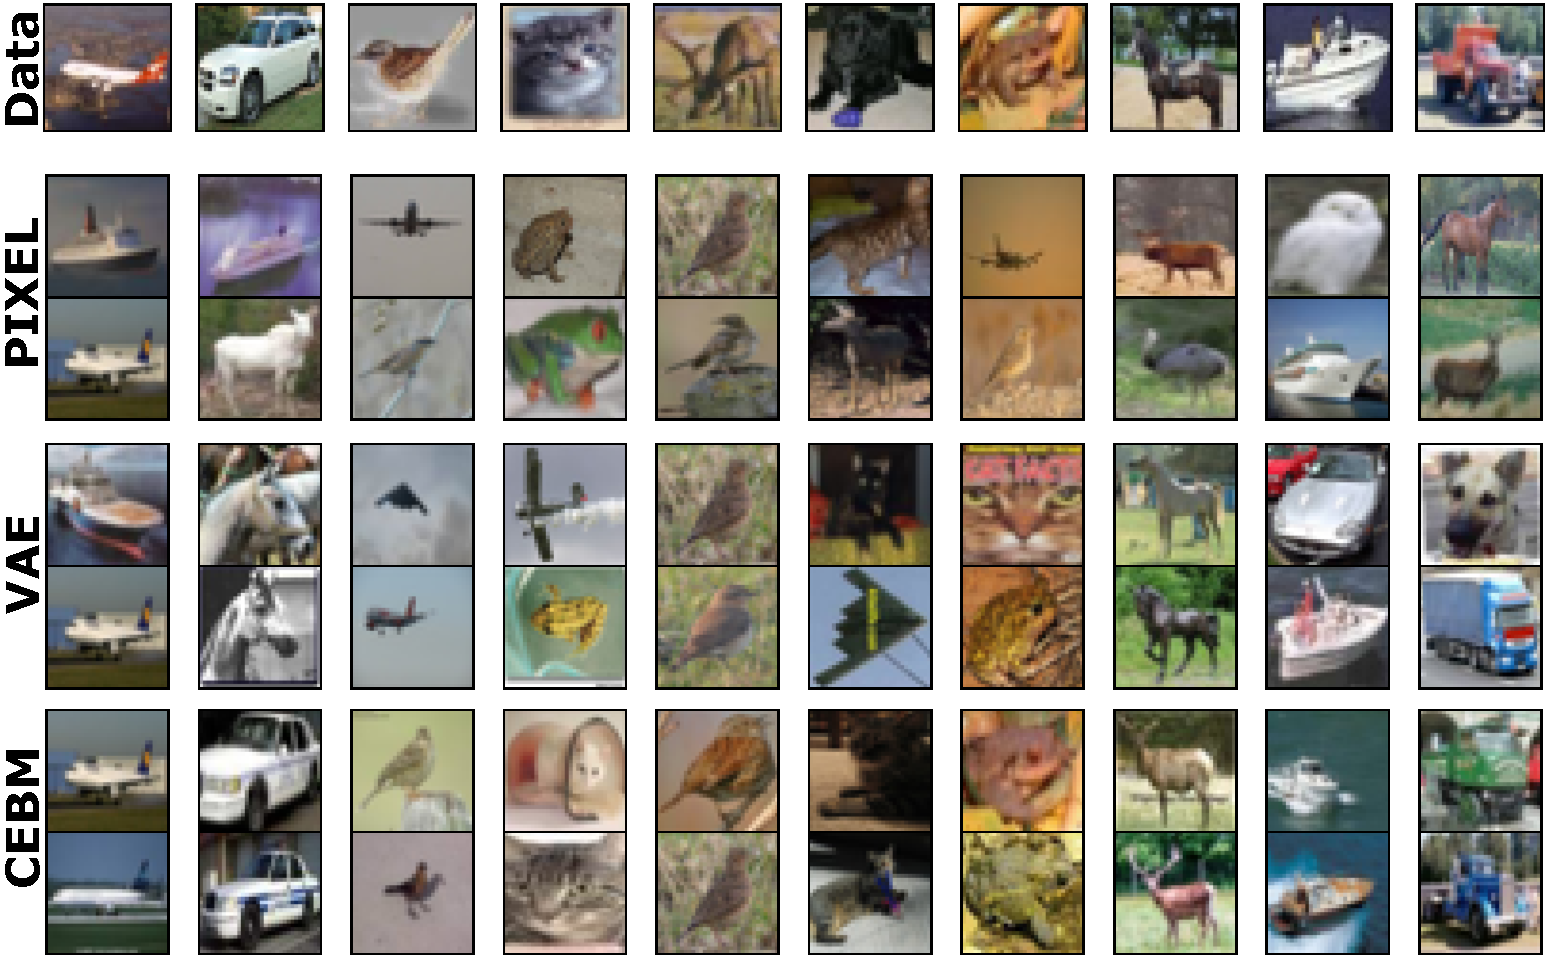
\includegraphics[width=0.45\linewidth]{figures/overview_figure.pdf}
\label{fig:nearest-neighbours}
}%
\subfigure[Confusion Matrices of 1-NN classification task on CIFAR10. Neighbors are defined by L2 distance in pixel space and latent space of CEBMs and VAEs. See Appendix~\ref{appendix-sec:confuion matrices} for more results.][]{
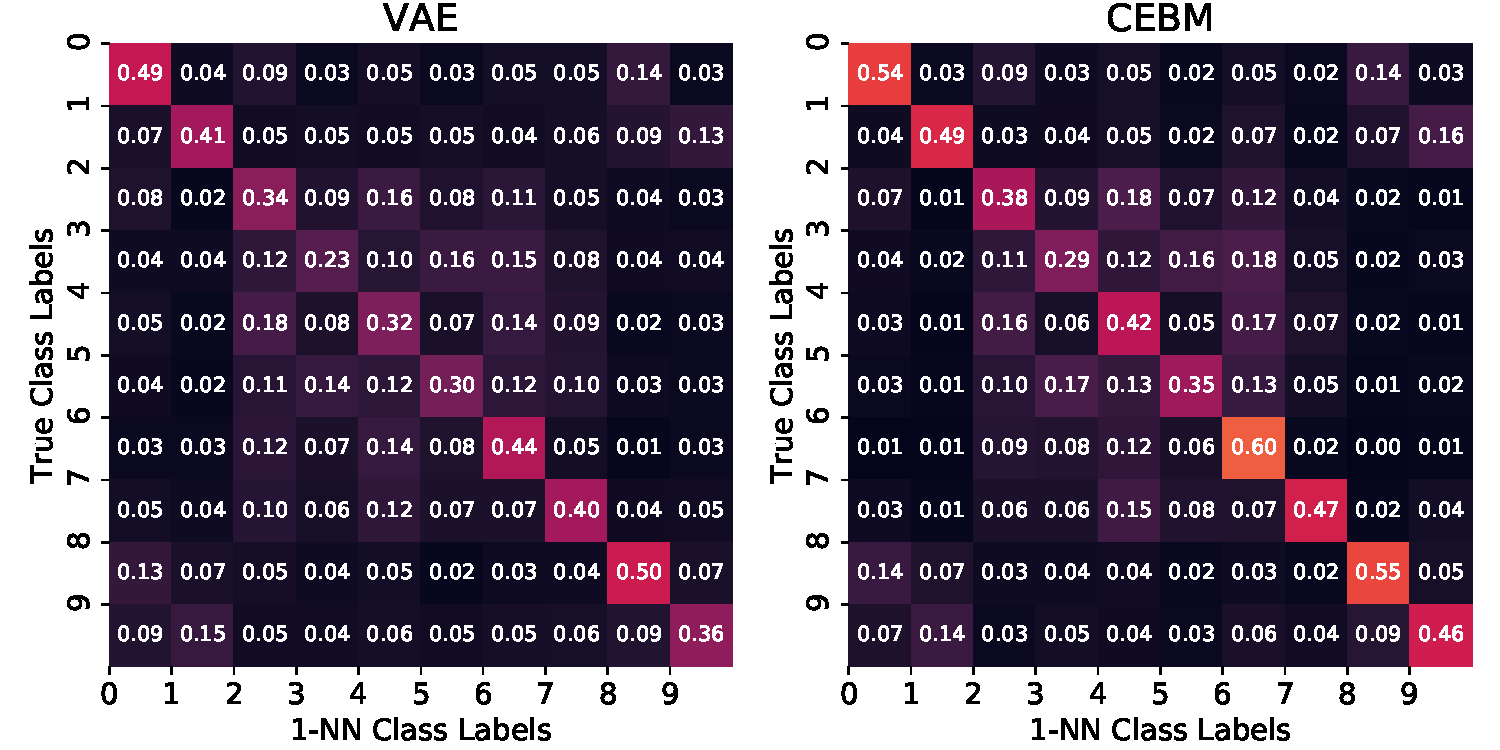
\includegraphics[width=0.5\textwidth]{figures/confusion_matrix_22row_cifar10.pdf}
\label{fig:cebm-confusion-matrices}
}
\caption{K-NN results using latent representations learned by CEBM on CIFAR-10.}
\end{figure*}
%\begin{comment}
% This leads us to consider the question whether it is possible to develop alternatives to VAE-based architectures that can be used to learning representations in a fully unsupervised manner, but do not rely on a generator that tries to faithfully reconstruct the input. It is possible that models that eliminate the requirement of a generator can learn more meaningful representations, in the sense that it becomes easier to discard factors of variation that give rise to variation in pixel space, but should be considered noise.
%\end{comment}


In this paper, we consider energy-based models (EBMs, \cite{du2019implicit, nijkamp2019anatomy, nijkamp2019learning}) as such an alternative to deep generative models. EBMs define an unnormalized density in terms of an energy function, which is a discriminative network rather than a generative network. We hope to learn more flexible densities that represents factors of variation at varying levels of precision.


% In this paper, we consider energy-based models (EBMs, \cite{du2019implicit}) as such an alternative to deep generative models. EBMs define an unnormalized density in terms of an energy function (typically a neural network); high energies correspond to lower probabilities. The energy function is defined as a discriminative network rather than a generative network. It takes pixels as input and returns a log probability. Since EBMs do not have a generator, we can hope to learn more flexible densities that represents factors of variation at varying levels of precision; the set of features that is needed to determine whether the background of an image is representative of the training data is likely smaller than the set of features that would fully encode all pixels in the background.



% %Since the energy function maps data to probabilities, EBMs are fundamentally discriminative m 
% %and produces a single value corresponding to the energy for that particular data. There are two main advantages from using EBMs over other generative models (in particular VAEs): (1) The generative model is more flexible given it is not explicitly defined. (2) There is only a single network to train. However, unlike VAEs, EBMs directly model the data; there is no notion of latent variable. This is ofcourse not necessarily a problem if our target application is image generation or density estimation. However, this can be problematic if our target application is to extract meaningful features from the data. Moreover, impose we may want to impose an inductive bias on the features we learn (e.g. disentangled representation).  

% %To date, EBMs have primarily been used to learn densities over training data \cite{}, or more generally class-conditional densities when labels are available \cite{}. 
More specifically, we propose conjugate EBMs (CEBMs), a new family of deep probabilistic models that combine a generative prior over latent variables with an energy-based likelihood. In CEBMs, the energy function defines a vector of sufficient statistics in a neural exponential family. While the normalizer of this family is intractable, we can nonetheless compute the posterior in closed form when we pair the likelihood with an appropriate conjugate prior. In this class of models the energy function fully determines both the marginal likelihood and the encoder, hereby side-stepping the need for a generator.


% %likelihood is an exponential family with an intractable normalizer. When we pair this likelihood with a matching conjugate prior, this results in a model with a tractable posterior. This means that if we train a CEBM by maximizing the marginal likelihood, the energy function fully determines both the marginal likelihood over training data 
% %In this paper, we propose conjugate EBMs (CEBMs): a new family of energy-based generative models that both have a flexible likelihood and allows for imposing an inductive bias on the latent space. Our proposed model defines a joint energy function on both the data and a latent variable. We show that how conjugacy can be exploited in order train the log marginal likelihood of the data by marginalising over the latent variable. 

% % We consider CEBMs with three types of priors. The first is a standard spherical Gaussian, which is common in the context of VAEs. We additionally consider two priors that combine continuous and discrete features. [TODO fix description; it is not clear to me what we mean by \emph{``For the first  extension, we show that how we can with a mixture model on the latent space. Second, we propose a Conjugate EBM that explicitly predicts both a discrete variable (class) and a continuous variable (style).''}] 

% We evaluate CEBMs To do so, we use class labels as an (imperfect) proxy for the primary factors of semantically significant variation in a dataset. 
In our experiments, we evaluate the representations learned by CEBM using class labels as a proxy for the primary factors of variation in a dataset. We show that CEBMs learn a notion of similarity that aligns closely with class labels in terms of the nearest neighbors in latent space (see Figure~\ref{fig:cebm-knn-cifar10}). Moreover, we show that the representations learned by CEBMs (in an unsupervised manner) give increased performance in few-shot learning and competitively performance in out-of-distribution detection tasks.

% We qualitatively and quantitatively evaluate the extent to which CEBMs can learn meaningful representations. To do so, we use class labels as an (imperfect) proxy for the primary factors of semantically significant variation in a dataset. We show that CEBMs learn a notion of similarity that aligns closely with class labels, in the sense that nearest neighbors in the latent space are more likely to belong to the same class. We quantify this result in few-shot learning experiments in which we train a classifier on a representation that was pre-trained without supervision. %Finally, we show that CEBMs yield improvements relative to VAE-based models in semi-supervised settings, where a limited number of labels are available during training of the model. 


% %The rest of the paper is structured as follows: In %Section \ref{sec:background} we provide an overview of %EBMs as well discussing the conjugacy relationship. We %then describe how conjugacy can be exploited to design %EBMs with latent variables in Section \ref{sec:cebm}. In %Section \ref{sec:related-work}, we discuss the relevant %prior work. Finally in Section \ref{sec:experiments}, we %perform a series of experiments on a variety of datasets %to demonstrate how our approach can both be used for %generating samples as well as learning a more meaningful %latent space compared to VAEs. 

% Our contributions can be summarized as follows:
% \begin{enumerate}[noitemsep,topsep=0pt,parsep=6pt,partopsep=0pt]
%     \item We propose CEBMs, a new class of energy-based models for unsupervised representation learning. CEBMs do not require a generator, unlike VAEs and GANs. Moreover, their joint density factorizes into a tractable posterior and an energy-based marginal over data. This means that CEBMs can be trained using existing methods for energy-based models in a manner that ensures that inference tractable at test time. 
%     \item We evaluate this new class of models by running experiments that test the extent to which CEBMs learn representations that agree with class labels (which are not used during training). We show that CEBMs learn a latent space in which neighbors are more likely to belong to the same class, which translates to increased performance in low-label downstream classification tasks, and that CEBMs also perform competitively in out-of-domain detection tasks.
% \end{enumerate}


% \vspace*{-1.0ex}
\section{Background}
\label{sec:background}
% \vspace*{-1.0ex}

\subsection{Energy-Based Models}
% \vspace*{-1.5ex}
An energy-based model~\cite{lecun2006tutorial} on a space of configuration $x\in\mathbb{R}^D$ defines a Gibbs-Boltzmann distribution as $p_\q(x) = {\exp \left\{- E_\q(x)\right\}} / {Z_\q}$.
$E_\q(x) : \mathbb{R}^D \xrightarrow[]{} \mathbb{R}$ is the energy function and maps each configuration to a scalar value. The normalizing constant $Z_\q = \int \!dx \: \exp \{- E_\q(x)\}$ is intractable in general.
To train an energy-based model, we maximize the expected log-likelihood as
\begin{align}
\label{eq:obj-ebm}
\mathcal{L}_{\q} 
&= \mathbb{E}_{p_\text{data}(x)}[\log p_\q (x)]
= \mathbb{E}_{p_\text{data}(x)}[-E_\q (x)] - \log Z_\q.
\end{align}
% The key difficulty when performing maximum likelihood estimation is that computing the gradient of $\log Z_\q$ is intractable. A common strategy is to express this gradient as an expectation with respect to $p_\q(x)$,
% \begin{align*}
%     \nabla \log Z_\q 
%     &= 
%     \mathbb{E}_{p_\q(x')}
%     \left[
%     -\nabla_\q E_\q(x')
%     \right]
%     ,
% \end{align*}
The gradient of $\mathcal{L}_\q$ has the form $\nabla_\q \mathcal{L}_{\q}
=
- \mathbb{E}_{p_\text{data}(x)}[\nabla_\q E_\q (x)] + \mathbb{E}_{p_\q(x')}[\nabla_\q E_\q(x')]
$.
% \begin{align*}
% %\label{eq:grad-ebm}
% \nabla_\q \mathcal{L}_{\q}
% &=
% - \mathbb{E}_{p_\text{data}(x)}[\nabla_\q E_\q (x)] + \mathbb{E}_{p_\q(x')}[\nabla_\q E_\q(x')]
% .
% \end{align*}
% Contrastive divergence methods \cite{hinton2002training} compute a Monte Carlo estimate of this gradient. This corresponds to \emph{maximizing} the probability of samples $x \sim p_\text{data}(x)$ from the data distribution and \emph{minimizing} the probability of samples $x' \sim p_\q(x')$ from the learned model. 

A common method for sampling from the model $x' \sim p_\q(x')$  is Stochastic 
Gradient Langevin Dynamics (SGLD)~\cite{welling2011bayesian}, which initializes a sample $x'_0 \sim p_0(x')$ and then performs a sequence of gradient updates with additional injected noise $\epsilon$
\begin{align}
\label{eq:sgld}
% &
% x'_0 \sim p_0(x')
% , \\
x'_{i+1} &= x'_i - \frac{\alpha}{2} \frac{\partial E_\q (x')}{\partial x'} + \epsilon
\,,&
\epsilon &\sim N(0, \alpha)
.
\end{align}
% SGLD is motivated as a discretization of a stochastic differential equation whose stationary distribution is equal to the posterior.
% It is correct in the limit $i \to \infty$ and $\alpha \to 0$, but in practice will have a bias. Moreover, it is common to independently tune the step size $\alpha$ and the variance of $\epsilon$ to allow for faster training~\cite{grathwohl2019your}.

% The initialization $x'_0$ is crucial because it determines the number of steps needed to converge to a high-quality sample. For this reason, EBMs are commonly trained \cite{nijkamp2019anatomy, du2019implicit, grathwohl2019your} using persistent contrastive divergence (PCD)~\cite{tieleman2008training}, which initializes some samples from a replay buffer $\mathcal{B}$ of previously generated samples.

% \subsection{Variational Autoencoders}
% \vspace*{-1.5ex}
% %Stochastic variational inference methods approximate the %posterior $p_\q(z | x)$ by learning a variational %distribution $q_\f(z | x)$ from some tractable family. 
% Variational autoencoders are a widely used class of deep generative models \cite{kingma2013auto-encoding, rezende2014stochastic}. A VAE defines a joint distribution $p_\q(\x, \z)$ over data $\x$ and latent variables $\z$; it combines an unstructured prior (e.g.~a spherical Gaussian) with a likelihood that is parameterized by an expressive neural network, often referred to as a decoder. An inference model, also known as an encoder, approximates the posterior $p_\q(\z \mid \x)$ by mapping each data point $x$ onto latent variables $z$. These models are trained by maximizing the stochastic evidence lower bound (ELBO) defined as
% %\vspace{-1.2em}
% \begin{align}
%     \label{eq:elbo}
%     \mathcal{L} (\f, \q)
%     &
%     = 
%     \mathbb{E}_{p_\text{data}(\x) \: q_\phi(\z \mid \x)}
%     \left[
%       \log \frac{p_\theta(\x, \z)}{q_\phi(\z \mid \x)}
%     \right] 
% \end{align}
% When the $q_\f(z|x)$ is reparameterizable, we can compute Monte Carlo estimates of the gradient of this objective using pathwise derivatives. Non-reparameterizable cases, such as models with discrete variables, require likelihood-ratio estimators~\cite{williams1992simple}.

% Despite their successes, VAEs have limitations. By maximizing the ELBO, we favor encoder-decoder pair that perfectly reconstruct their input, so there is nothing preventing the VAE from mapping similar inputs to similar encoding, even when they might be semantically different. Likewise, examples that might be very dissimilar in pixel space because of noise or benign transformations might end up with very different latent representations. 

\subsection{Conjugate Exponential Families}
\vspace*{-1.5ex}
An exponential family is a set of distributions whose probability density function or probability mass function can be expressed in the following form.
\begin{align}
\label{eq:cebm-likelihood}
    p(\x \mid \eta) 
    &= 
    h(\x) \exp \big\{ 
        t(\x)^\top \eta   
        - A(\eta) \big\}.
\end{align}
% where $h(\cdot)$ is a vector of natural parameters $\eta$, a vector of sufficient statistics $t(\cdot)$, and a log normalizer $A(\cdot)$.
% If a likelihood belongs to an exponential family, then there exists a conjugate prior, that is, a distribution whose general form is not changed by multiplication with the likelihood and normalization. It is common for conjugate priors to also belong to some exponential family, with the following form.

where $h(\cdot)$ is a vector of natural parameters $\eta$, a vector of sufficient statistics $t(\cdot)$, and a log normalizer $A(\cdot)$.
If a likelihood belongs to an exponential family, then there exists a conjugate prior with the form  $p(\eta \mid \lambda) = h_0(\eta) \exp \big\{ t_0(\eta)^\top \lambda - A_0(\lambda) \big\}$.
% \begin{align*}
%     p(\eta \mid \lambda) 
%     &= 
%     h_0(\eta) \exp \big\{ 
%     t_0(\eta)^\top \lambda
%     - A_0(\lambda) \big\}.
% \end{align*}   
A prior is conjugate to a likelihood when its vector of sufficient statistics comprises the natural parameters and the log-normalizer of the likelihood $t_0(\eta) = \big[ \eta, - A(\eta) \big]$, $\lambda = \big[ \lambda_1, \lambda_2 \big]$.
% \begin{align*}
% % \label{eq:sufficient-stats}
%     t_0(\eta) &= \big[ \eta, - A(\eta) \big], 
%     &
%     \lambda &= \big[ \lambda_1, \lambda_2 \big].
% \end{align*}
The convenient property of conjugate exponential families is that both the marginal likelihood $p(x \mid \lambda)$ and the posterior $p(\eta \mid x, \lambda)$ are tractable. The reason is that the joint probability has the form
\begin{align*}
    p(x, \eta \mid \lambda) = p(x \mid \eta) \: p(\eta \mid \lambda)
    =\exp \big\{ 
      \eta^\top \! \big(\lambda_1 \!+\! t(x)\big) 
      -
      A(\eta) (\lambda_2 \!+\! 1) 
      -
      A_0(\lambda)
    \big\}.
\end{align*}
If we substitute $\tilde{\lambda}_1 = \lambda_1 + t(x)$ and $\tilde{\lambda}_2 = \lambda_2 + 1$, we can equivalently factorize this joint as
\begin{align}
    \label{eq:cef-joint}
    \begin{split}
    p(x, \eta \mid \lambda) = p(\eta \mid x, \lambda) \: p(x \mid \lambda) 
    = p(\eta \mid \tilde{\lambda}) \: \exp\big\{ A_0(\tilde{\lambda}) - A_0(\lambda) \big\}.
    \end{split}
\end{align}
This shows that the posterior is in the same exponential family as the prior, and that we can express the marginal likelihood using the log normalizer $A_0(\cdot)$
\begin{align}
    \label{eq:cef-posterior-and-marginal}
    p(\eta \mid x, \lambda) &= p(\eta \mid \tilde{\lambda}),
    &
    p(x \mid \lambda) &= \exp\big\{ A_0(\tilde{\lambda}) - A_0(\lambda) \big\}.
\end{align}
% In general both the log normalizer for an arbitrary vector of sufficient statistics $t(x)$ and the conjugate prior are intractable, since they require solving the following integrals
% % \begin{align*}
% %     A(\eta) = \log \int dx \: \exp \big\{ t(x)^\top \eta  \}.
% % \end{align*}
% \begin{align*}
%     &A(\eta) = \log \int dx \: \exp \big\{ t(x)^\top \eta  \}, &A_0(\lambda) = \log \int d\eta \: \exp \big\{ \lambda_1^\top \eta - \lambda_2 A(\eta) \big\}.
% \end{align*}
%
% JWM: WROTE THIS WHOLE BIT BUT GOT RID OF IT. I THINK IT CONFUSES MORE THAN IT HELPS 
%

% In deep generative models, we can define an exponential family likelihood $p_\q(x \mid \eta_\q(z))$ in terms of a generator network $\eta_\q(z)$ that maps latent variables $z$ to a vector of natural parameters. This is in fact normal practice, since VAEs generally use a Gaussian or a Bernoulli likelihood, which are both exponential family distributions. However the corresponding conjugate prior $p_\q(z \mid \lambda)$ is intractable. This prior would have sufficient statistics $t_0(z) = [\eta_\q(z), -A(\eta_\q(z))]$ that are defined in terms of the generator network, which means that we cannot compute its log normalizer
% \begin{align}
%     A_0(\lambda) = \log \int dz \: \exp \big\{ \lambda_1^\top \eta_\q(z) - \lambda_2 A(\eta_\q(z)) \big\}. 
% \end{align}


%%%%%%%%%%%%%%%%%%%%%%%%%%%%%%%%%%%%%%%%%%%%%%%%%%%%%%%%%%%%%%%%%%%%%%%%%%%%%%%%%%%%%%%%%%%%%%%%%%%%%%%%%
\section{Conjugate Energy-Based Models}
\label{sec:cebm}
% \vspace*{-2.0ex}
%%%%%%%%%%%%%%%%%%%%%%%%%%%%%%%%%%%%%%%%%%%%%%%%%%%%%%%%%%%%%%%%%%%%%%%%%%%%%%%%%%%%%%%%%%%%%%%%%%%%%%%%%
% In this Section, we show that we can design energy functions such that the latent variable can be marginalized over by relying on the conjugacy relationship. Given a data point $\vx$, let $T_{\q}(\vx)$ be a set of sufficient statistics for data $\vx$. 

%To learn structured representations of the data $x$, we will design an energy-based %model that incorporates a latent space of $z$. Instead of learning reconstruction of %$z$ at the level of pixel space, we learn a 'relaxed likelihood' that measures the %agreement between data and latent variables at an intermediate level of %representation. Here we consider an unnormalized density

In this paper we are interested in learning a probabilistic model that defines a joint distribution $p_\q(x, z)$ over high-dimensional data $x \in \mathbb{R}^D$ and a lower-dimensional set of latent variables $z \in \mathbb{R}^K$. Because most work on deep generative models has focused on images, we will restrict ourselves to this data modality. 

%Our goal is to learn a model in which latent variables $z$ reflect high-level features of interest, rather than low-level features that we might consider nuisance variables. 
The intuition that guides our work is that we would like to measure agreement between latent variables and data at a high level of representation, rather than at the level of individual pixels, where it may be more difficult to distinguish informative features from noise. To this end, we will explore energy-based models as an alternative to models that learn a generator network.
Concretely, we propose to consider models of the form
\begin{align}
    &p_\q(x, z) = \frac{1}{Z_\q}\: \exp \big\{ -E_\q(x,z)\big\}, & E_\q(x,z) = -t(x)^\top \eta_\q(z) - b_\q(z).
\end{align}
where $\q$ are the parameters of our model, $Z_\q$ is the partition function. $\eta_\q: \mathbb{R}^K \to \mathbb{R}^H$ plays a role similar to that of a generator, which maps latent variables to a vector of natural parameters of dimension $H$. $t: \mathbb{R}^D \to \mathbb{R}^H$ plays the role of an encoder, which maps data to a vector of sufficient statistics. The term $b_\q: \mathbb{R}^K \to \mathbb{R}$ serves as an inductive bias that plays a role analogous to the prior.Our intuition is that controlling the dimension $H$ may allow us to define energy functions that reflect agreement at a higher or lower level of representation. 
The generative model in a VAE can be recovered as a special case (see Appendix~\ref{appendix:sec-vae-special-case}). 

% In the middle of the spectrum, we could define a form
% \begin{align}
%     E_\q(x, z) = -t_\q(x)^\top \eta_\q(z) - b_\q(z).
% \end{align}
% Here, statistics at an intermediate level of representation are computed using a discriminative encoder network $t_\q(x)$, and natural parameters at the same intermediate level of representation are computed using a generator network $\eta_\q(z)$. The bias $b_\q(z)$ could take the form of a neural energy function, the logarithm of a deep generative prior $\log p_\q(z)$, or a combination of the two. This class of energy functions is the most general, in the sense that it allows us to define notions of agreement at varying levels of intermediate representation. However, these models may also be the most difficult to train, since both conditionals and marginals in the model will be intractable.
%
In general, we can define the energy in terms of an encoder network $t_\theta(x)$ that maps high-dimensional data to a low-dimensional vector of sufficient statistics. We combine this encoder with a bias $b_\q(z) = \log p_\q(z \mid \lambda)$ in form of a tractable exponential family with $\eta(z)$, 
\begin{align}
    b_\q(z) = \eta_\q(z)^\top \lambda - A(\lambda).
\end{align}
We can then define the energy function 
\begin{align}
    \begin{split}
    E_\q(x, z) = -t_\q(x)^\top \eta_\q(z) - b_\q(z),
               = - \big(\lambda + t_\q(x) \big)^\top \eta_\q(z) + A(\lambda).
    \end{split}
\end{align}
This form of the energy function has a very convenient property: It corresponds to a model $p_\theta(x,z)$ in which the posterior $p_\theta(z \mid x)$ is tractable. To see this, we can make a substitution $\tilde{\lambda} = \lambda + t_\q(x)$ analogous to the one in Equation~\ref{eq:cef-joint}, which allows us to express the energy as
\begin{align*}
    \begin{split}
    E_\q(x, z) &= -\big(\eta_\q(z)^\top \tilde{\lambda}  - A(\tilde{\lambda}) \big) -\big(A(\tilde{\lambda}) - A(\lambda) \big) 
    \end{split}
\end{align*}
We now see that we can factorize the corresponding density $p_\q(x,z) = \exp \{ - E_\q(x,z) \} / Z_\q$, 
\begin{align}
    p_\q(x,z \mid \lambda) 
    &= 
    p_\q(x \mid \lambda) \: p_\q(z \mid x, \lambda).
\end{align}
which yields a posterior and marginal that are analogous the distributions in Equation~\ref{eq:cef-posterior-and-marginal},
\begin{align}
    p_\q(z \mid x, \lambda) = p(z \mid \lambda + t_\q(x)), \:
    p_\q(x \mid \lambda) = \frac{1}{Z_\q} \exp\big\{ A\big(\lambda + t_\q(x) \big) - A\big(\lambda\big) \big\}.
\end{align}
In other words, the joint density of this model factorizes into an intractable energy-based marginal likelihood $p_\theta(x \mid \lambda)$ and a tractable posterior $p_\theta(z \mid x, \lambda)$. This posterior is conjugate, in the sense that it is in the same exponential family as the bias. For this reason, we refer to this class of models as conjugate energy-based models (CEBMs).

CEBMs differ from VAEs in that they lack a generator network. Instead, the density is fully specified by the encoder network $t_\theta(x)$, which defines a notion of agreement $(\lambda + t_\q(x))^\top \eta(z)$ between data and latent variables in a low-dimensional feature space.  

In addition to having a tractable posterior, CEBMs have the convenient property that the marginal likelihood $p_\q(x \mid \lambda)$ itself can be expressed as an energy-based model that is defined in terms of the log normalizer $A(\cdot)$ and the encoder network $t_\q(x)$. This means that we can train CEBMS by maximizing the marginal likelihood $p_\q(x \mid \lambda)$ using persistent contrastive divergence (see~Algorithm~\ref{alg:cebm})~\cite{tieleman2008training}, in the same way that other EBMs are trained~\cite{nijkamp2019anatomy, du2019implicit,grathwohl2019your}. 
% \vspace*{-0.5ex}
\section{Inductive Biases}
% \vspace*{-0.5ex}
CEBMs have a property that is somewhat counter-intuitive: While the posterior in $p_\q(z \mid x, \lambda)$ in this class of models is tractable, the prior $p_\q(z)$ is in general not tractable. In particular, although the bias $b_\q(z)$ is the logarithm of a tractable exponential family, it is not the case that $p_\q(z) \not= \exp \{-b_\q(z) \}$. Rather the prior $p_\q(z)$ has the form,
\begin{align*}
    p_\q(z) = \frac{\exp \{-b_\q(z)\}}{Z_\q} \ \int \! dx \: \exp \{t_\q(x)^\top \eta(z) \}.
\end{align*}
% In other words, the term $b_\q(z)$ defines an inductive bias, but this bias is different from the bias in a VAE, where the prior is always tractable by construction.\footnote{Concretely, the bias in a VAE (Eq.~\ref{eq:vae-bias}) contains the log prior $\log p_\q(z)$ and the log normalizer $A(\eta_\q(z))$ of the likelihood. In a CEBM, by contrast, we omit the second term $A_\q(\eta(z)) = \log \int dx \exp \{ t_\q(z)^\top \eta(z) \}$, which is intractable, and hereby implicitly incorporate it into the prior.} 


% \begin{figure}[!t]
% \centering
% 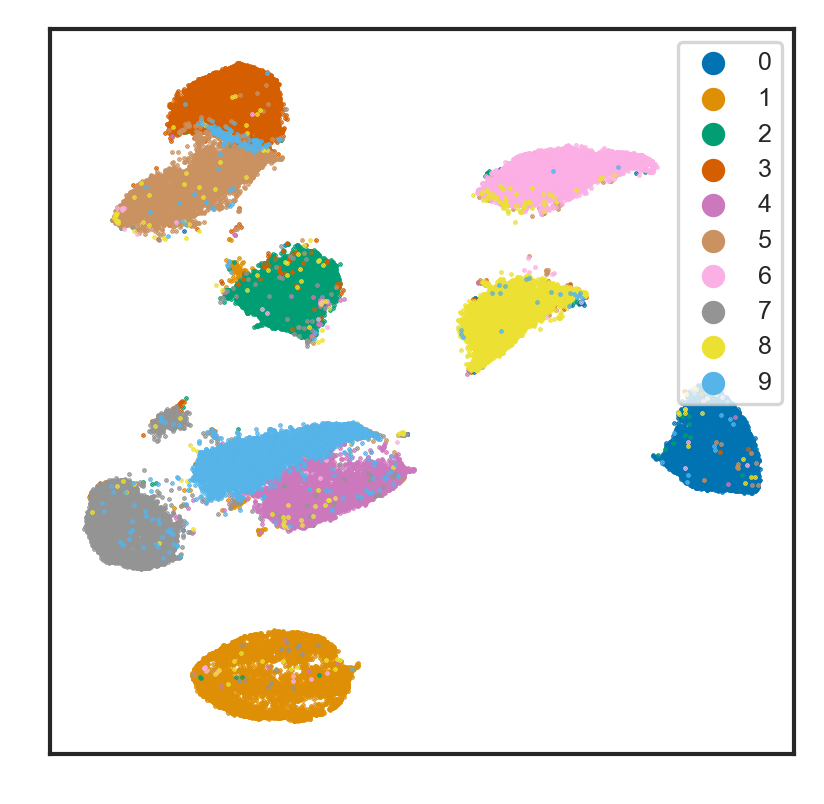
\includegraphics[width=0.225\linewidth]{figures/mnist_cebm_z_space.png}
% 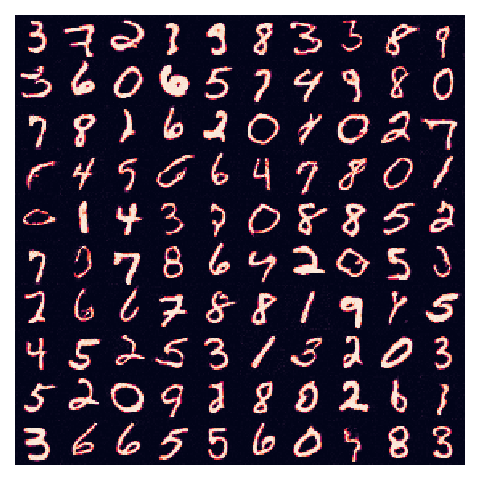
\includegraphics[width=0.225\linewidth]{figures/mnist_cebm_buffer_samples.pdf}
% \vspace*{-1.5ex}
% \caption{CEBM trained on MNIST; (\emph{Left}) latent space visualized with UMAP~\cite{mcinnes2018umap}. (\emph{Right}) Random samples generated from the model.}
% %\vspace*{-1.5ex}
% \label{fig:cebm-mnist}
% \end{figure}


%The bias in a VAE (Equation~\ref{eq:vae-bias}) differs from the bias in a CEBM in that it contains the log-normalizer of the likelihood in addition to the logarithm of the prior. In a CEBM we cannot compute this log-normalizer, since the integral with respect to $x$ will be intractable. For this reason, the term $b_\q(z)$ acts as an inductive bias, but this inductive bias does not constrain the learned representation in the same way as in a VAE, where the prior $p_\q(z)$ is tractable by construction. 

In principle the bias a CEBM can take the form of any exponential family distribution. Since products of exponential families are also in the exponential family, this covers a broad range of possible biases. In this paper, we will constrain ourselves to Spherical Gaussian and Mixture of Gaussians. We provide derivations for both cases in Appendix~\ref{appendix-sec:inductive-bias}.




% So far we have shown that we can impose a Gaussian inductive bias on the latent space of CEBMs. However, one can argue that such inductive bias is too simple for most real-world datasets. Here, we ask the following question: can we impose a more structured inductive bias (e.g. a mixture model) on the latent space? It turns out that the answer is yes. Below, we will describe how to design such energy functions where the inductive bias on $z$ is a mixture model while we still are able to marginalize over it. 
% % We show that we can use the same conjugacy trick to design CEBMs where $\gamma_{\q}(x)$ can be computed analytically while the inductive bias on the latent space is a Gaussian mixture model.

% Let $y$ and $K$ be the cluster assignment, and the total number of clusters respectively. For simplicity, let's assume that every cluster has an equal probability of $\frac{1}{K}$. We now define the joint distribution over $z$ and $y$ as:
% \begin{equation}
% p(z, y \mid \lambda) = \frac{1}{K}\prod_{k=1}^{K}p(z \mid y=k,\lambda)^{I[y=k]}
% \end{equation}
% where $I$ is the identity function. We can re-write this distribution in an exponential form:
% \begin{equation}
% \label{eq:gmm-cebm-prior}
% \frac{1}{K} h(z) \exp \{\sum_{k=1}^K I[y=k]\left(\lambda^{T}_{k} t(z) - A_{0}(\lambda_{k})\right)\}
% \end{equation}
% where $\lambda_k$ is the natural parameters for the $k$'th mixture. The likelihood will have the same format as Eq.~\ref{eq:cebm-likelihood}. However, we can re-write the likelihood in a way to be conjugate to Eq.~\ref{eq:gmm-cebm-prior}:
% \begin{align}
% \gamma(x \mid z, y) 
% &= 
% \exp \{ \eta(z)^\top t_\q(x) \} \\
% &= \exp \{\sum_{k=1}^{K} I[y=k]\eta(z)^\top t_\q(x) \}
% \end{align}
% We now write the joint probability distribution over $x$, $z$, and $y$ as:
% \begin{align}
% \label{eq:cebmm-joint}
% p_{\q}(x,y,z)
% &=
% \frac{\gamma_{\q}(x,y,z)}{Z}
% \\
% \gamma_{\q}(x,y,z)
% &=
% \gamma_{\q}(x|y,z)p(z,y) 
% \end{align}
% This yield posterior distribution $p_{\q}(z|x,y)$ as:
% \begin{align}
% h(z)\exp \big\{\sum_{k=1}^{K} I[y=k]\left((\lambda_{k} + t_{\q}(x))^\top t(z) - A_{0}(\lambda_{k} + t_{\q}(x))\right) \big\}.  
% \end{align}
% and $\gamma_{\q}(x,z)$ as:
% \begin{align}
% \frac{1}{K}\exp \big\{ \sum_{k=1}^{K} I[y=k] \left(A_{0}(\lambda_k + t_{\q}(x)) 
%  - A_{0}(\lambda_k) \right) \big\}
% \end{align}
% By marginalizing over $y$, we can define $E_{\q}^{\textsc{CEBMM}}(x)$ as:
% \begin{equation}
% E_{\q}(x) = \frac{1}{K} \sum_{k=1}^{K} \exp \{A_{0}(\lambda_k + t_{\q}(x)) -  A_{0}(\lambda_k) \}
% \end{equation}

%%%%%%%%%%%%%%%%%%%%%%%%%%%%%%%%%%%%%%%%%%%%%%%%%%%%%%%%%%%%%%%%%%%%%%%%%%%%%%%%%%%%%%%%%%%%%%%%%%%%%%%%%

% \citet{nijkamp2019anatomy, nijkamp2019learning} performed a comprehensive analysis of convergence in recent EBMs, where they study a variety of factors such as MCMC chain initialization, network, and optimizer. They identify that critical factors for diagnosing these models differ between the energy of positive and negative samples. Many of these findings were helpful during the training and evaluation of EBMs in our work. The same authors show that it is sometimes possible to learn a valid model even generate realistic samples even with a non-convergent, non-mixing short-run MCMC sampling  \cite{nijkamp2019learning}. 

% %%%%%Hao's Edit Starts%%%%%%%
% % talked about all ancient work before I was born...
% The first modern EBMs with energy functions as deep neural networks that were able to generate realistic samples with Langevin sampling were introduced by \citet{du2019implicit,xie2016theory}.
% \citet{nijkamp2019anatomy, nijkamp2019learning}
% %%%%%Hao's Edit Ends%%%%%%%%

%%%%%%%%%%%%%%%%%%%%%%%%%%%%%%%%%%%%%%%%%%%%%%%%%%%%%%%%%%%%%%%%%%%%%%%%%%%%%%%%%%%%%%%%%%%%%%%%%%%%%%%%%
\vspace*{-0.5ex}
\section{Related Work}
\label{sec:related-work}
\vspace*{-1.5ex}
%%%%%%%%%%%%%%%%%%%%%%%%%%%%%%%%%%%%%%%%%%%%%%%%%%%%%%%%%%%%%%%%%%%%%%%%%%%%%%%%%%%%%%%%%%%%%%%%%%%%%%%%%
Energy-based models \cite{lecun2006tutorial} have a long history in machine learning. Recent work on EBMs has shown that it is possible to use deep neural network as energy functions, and that it is possible to use Langevin methods to generate realistic samples from learned models \cite{nijkamp2019anatomy, nijkamp2019learning, du2019implicit,xie2016theory}. Work by \citet{grathwohl2019your} interprets classifiers through the lens of energy-based models. \citet{liu2020hybrid} propose a similar model where the objective combines a discriminative conditional and a generative conditional conditional distribution.
%%%%%%%%%%%%%%%%%%%%%%%%%%%%%%%%%%%%%%%%%%%%%%%%%%%%%%%%%%%%%%%%%%%%%%%%%%%%%%%%%%%%%%%%%%%%%%%%%%%%%%%%%

\vspace*{-0.5ex}
\section{Experiments}
\label{sec:experiments}
% \vspace*{-1.5ex}
%%%%%%%%%%%%%%%%%%%%%%%%%%%%%%%%%%%%%%%%%%%%%%%%%%%%%%%%%%%%%%%%%%%%%%%%%%%%%%%%%%%%%%%%%%%%%%%%%%%%%%%%


\begin{figure*}[!t]
\centering
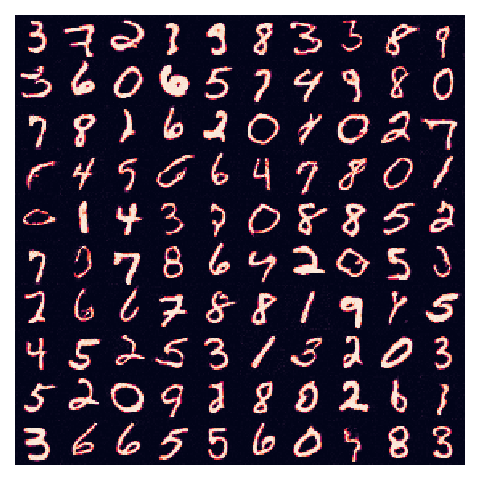
\includegraphics[width=0.205\textwidth]{figures/mnist_cebm_buffer_samples.pdf}
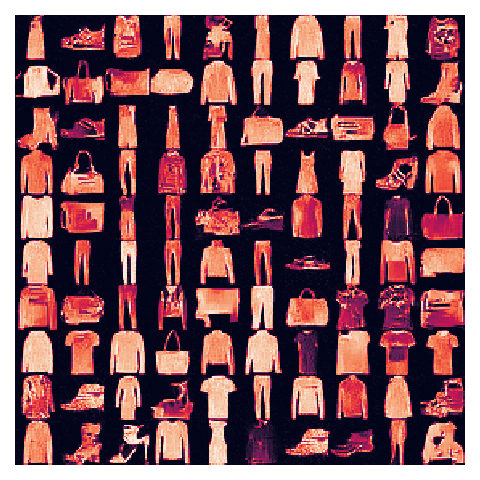
\includegraphics[width=0.205\textwidth]{figures/fmnist_cebm_samples.pdf}
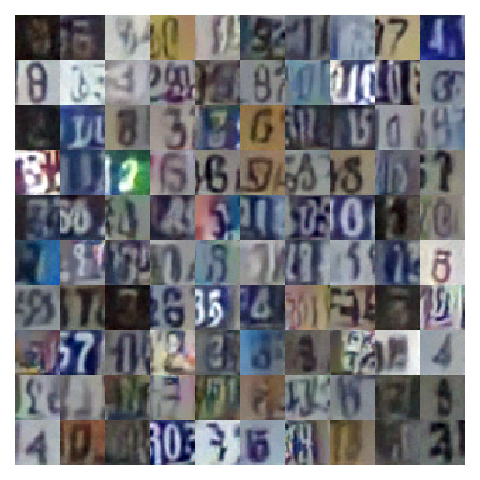
\includegraphics[width=0.205\textwidth]{figures/svhn_cebm_buffer_samples3.pdf}
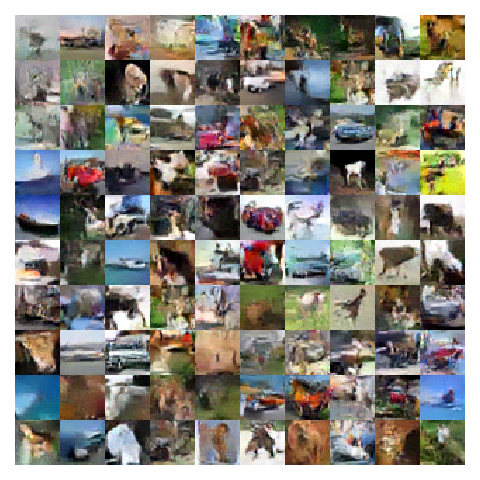
\includegraphics[width=0.205\textwidth]{figures/cifar10_cebm_buffer_samples.pdf}
\vspace*{-1.5ex}
\caption{CEBM Samples of MNIST, F-MNIST, SVHN and CIFAR-10.}
%\vspace*{-1.5ex}
\label{fig:generated-samples}
\end{figure*}

% Our experiments evaluate to what extent CEBMs can learn representations that encode meaningful factors of variation, whilst discarding details about the input that we would consider noise. This question is difficult to answer in generality, and in some sense not well-posed; whether a factor of variation should be considered signal or noise can depend on context. For this reason,
% Our experiments focus on the extent to which representations in CEBMs can recover the multimodal structure in datasets that are used for classification. %(MNIST~\cite{lecun1998gradient}, Fashion-MNIST~\cite{xiao2017fashion}, SVHN~\cite{netzer2011reading}, and CIFAR-10~\cite{krizhevsky2009learning}). 
% While class labels are an imperfect proxy, they provide a means of quantifying differences between representations that were learned in an unsupervised manner.
% We begin with a qualitative evaluation by visualizing samples. We then demonstrate that learned representations align with class structure, in the sense that nearest neighbors in the latent space are more likely to belong to the same class (Section~\ref{sec:exp:quality}). In addition, we measure few-shot classification accuracy for representations that were pre-trained without supervision (Section~\ref{sec:exp:fewshots}).






% \textbf{Models:}
% \begin{enumerate}
% \item $\gamma(\vx|\vz) = \text{exp}\left(\vz^{T}t_{\vtheta}(\vx) - (\vz^{2})^{T}t_{\vtheta}(\vx)^{2}\right)$
% \item $\gamma(\vx | \vz) = \text{exp}\left(\vz^{T}t_{\vtheta}(\vx) - (\vz^{2})^{T}t_{\vtheta}(\vx)^{2}\right) \\ p(\vz, \vy) = \frac{1}{K}\prod_{k}p(z|y=k)^{i[y==k]}$
% \item $\gamma(\vx| \vz, \vy) = \text{exp}\left(\vz^{T}t_{\vtheta}(\vx) - (\vz^{2})^{T}t_{\vtheta}(\vx)^{2}\right) \\ \text{exp}\left(f_{\q}(\vx)[y]\right)  \quad p(\vz, \vy) = p(\vz) p(\vy)$
% \item $\gamma(\vx| \vz, \vy) = \text{exp}\left(\vz^{T}t_{\vtheta}(\vx, \vy) - (\vz^{2})^{T}t_{\vtheta}(\vx, \vy)^{2}\right) \\ \text{exp}\left(f_{\q}(\vx)[y]\right)$
% \end{enumerate}


% \subsection{Latent Space Quality}

% In order to assess the quality of the latent space in CEBMs, we train a classifier on the training latent variables. Our results show that CEBMs can indeed learn a more meaningful latent space compared to VAEs.

\setlength{\tabcolsep}{5pt}
\begin{table*}[!t]
\scriptsize
\centering
%\vspace*{-1.5ex}
\begin{tabular}{l|cccc|cccc|cccc|cccc}
\toprule
 & \multicolumn{4}{c}{MNIST} & \multicolumn{4}{|c}{Fashion-MNIST} & \multicolumn{4}{|c}{CIFAR-10} & \multicolumn{4}{|c}{SVHN}\\
Models & $1$ & $10$  & $100$ & $full$ & $1$ & $10$  & $100$ & $full$ & $1$ & $10$  & $100$ & $full$ & $1$ & $10$  & $100$ & $full$ \\
\midrule
\midrule
VAE & 42 & 85 & 92 & 95 & 41 & 63 & 72 & 81 & 16 & 22 & 31 & 38 & \textbf{13} & 13 & 16 & 36\\
GMM-VAE & 53 & 86 & 93 & 97 & 49 & 68 & 79 & 84 & \textbf{19} & 23 & 33 & 39 & \textbf{13} & 14 & 23 & 56  \\
\midrule
IGEBM & 63 & 89 & 95 & 97 & 50 & 70 & 79 & 83 & 16 & 26 & 33 & 42 & 10 & 16 & 35 & 49\\
CEBM & \textbf{67} & 89 & 95 & 97 & \textbf{52} & 70 & 77 & 83 & \textbf{19} & \textbf{30} & \textbf{42} & \textbf{52} & 12 & \textbf{25} & \textbf{48} & \textbf{70}\\
CEBMM & \textbf{67} & \textbf{91} & \textbf{97} & \textbf{98} &\textbf{52} & \textbf{71} & \textbf{80} & \textbf{85} & 16 & 28 & \textbf{42} & 51 & 10 & 17 & 39 & 60 \\
\bottomrule
\end{tabular}
\label{tab:few-shot classification}
\caption{Few-Shot classification accuracy. We pre-train 5 unsupervised models (rows) on MNIST, Fashion-MNIST, CIFAR10, SVHN. Then we train logistic classifiers using 1, 10, 100 examples per class (i.e. shots) and the full training dataset. We report the testing classification accuracy, where CEBM outperforms.}
\end{table*}

% \vspace*{-1.5ex}

\setlength{\tabcolsep}{4pt}
\begin{table*}[!h]
\scriptsize
\centering
\begin{tabular}{l|ccc|ccc||ccc|ccc}
\toprule
& \multicolumn{6}{c||}{Fashion-MNIST} &    \multicolumn{6}{c}{CIFAR-10}\\
& \multicolumn{3}{c|}{$\log p_{\q}(\vx)$} & \multicolumn{3}{c||}{$\| \nabla_{\vx}\log p_{\q}(\vx)\|$} &  \multicolumn{3}{c|}{$\log p_{\q}(\vx)$} & \multicolumn{3}{c}{$\| \nabla_{\vx}\log p_{\q}(\vx)\|$}\\
\midrule
            &  MNIST  & E-MNIST& C &  MNIST & E-MNIST & C &  SVHN & Texture & C &  SVHN & Texture & C \\
\midrule
VAE         & 50 & 39 & 9 & 61 & 57 & 1  & 42 & \textbf{58} & 41 & 38 & \textbf{51} & 37 \\
IGEBM       & 35 & 36 & 90 & 78 & 82 & 96& 45 & 31 & 64 & 33 & 17 & \textbf{62} \\
CEBM        & 37 & 34 & 90 & \textbf{82} & \textbf{89} & \textbf{98} & 47 & 32 & \textbf{66} & 31 & 17 & 54 \\
CEBMM       & \textbf{56} & \textbf{56} & \textbf{92} & 56 & 80 & 95     & \textbf{55} & 30 & 62 & \textbf{40} & 23 & \textbf{62}  \\
\bottomrule
\end{tabular}
\caption{AUROC scores in OOD Detection. We use $\log p_{\q}(\vx)$ and $\| \nabla_{\vx}\log p_{\q}(\vx)\|$ as score functions.The left block shows results of the models trained on F-MNIST and tested on MNIST, E-MNIST, Constant (C); The right block shows results of the models trained on CIFAR-10 and tested on SVHN, Texture and Constant (C).}
\label{tab:ood-detection}
\end{table*}

\subsection{Samples and Latent Space}
\label{sec:exp:quality}
% \vspace*{-1.5ex}
% As with other EBMs~\cite{du2019implicit}, we can use SGLD to sample from CEBM. In Figures~\ref{fig:generated-samples} \&~\ref{fig:cebm-mnist}, we show generated samples from CEBM trained on different datasets by running 500 steps of SGLD. Even though the sample quality in CEBMs is far from state-of-the-art generative models, we observe that CEBMs do not suffer from blurriness as VAEs. Furthermore, these sample show that CEBMs are able to do a reasonable job at approximating the data distribution.

% Recent work has often focused on EBMs as an alternative to generative models~\cite{du2019implicit, nijkamp2019anatomy}, where it is natural evaluate model performance in temrs of the the quality of generated samples. While generation is not our intended use case in this paper, such samples do serve as a useful diagnostic, in the sense that they allow us to visually inspect what characteristics of the input data are captured by the learned representation. 

We train our models with both inductive biases and call them as CEBM (Spherical Gaussian) and CEBMM(Mixutre of Gaussian). See Appendix~\ref{appendix-architectures} and Appendix~\ref{appendix-sec:training-details} for architecture and training details. We begin with a qualitative evaluation by visualizing samples. Figures~\ref{fig:generated-samples} shows samples by CEBMs with uniform noise initialization an 500 SGLD steps. 
% While generation is not our intended use case in this paper, such samples do serve as a useful diagnostic, in the sense that they allow us to visually inspect what characteristics of the data are captured by the representation. 
% The distribution over images is diverse and captures the main characteristics of the input data. 
% Sample quality is roughly on par with samples from other EBMs \cite{nijkamp2019anatomy}, although it is possible to generate samples with higher visual quality using class-conditional EBMs~\cite{du2019implicit, grathwohl2019your, liu2020hybrid} (which assume access to labels).

% For a quantitative assessment, we report Frechet Inception Distance (FID)~\cite{heusel2017gans} where we compare against Glow~\cite{kingma2018glow}, GMM-VAE~\cite{tomczak2018vae}, and IGEBM~\cite{du2019implicit}. As shown in Table~\ref{tab:fid-scores}, CEBM is able to achieves a competitive FID score. 

To assess to what extent the representation in CEBMs aligns with classes in each dataset, we look at the agreement between the label for each data point and the label of its nearest neighbor in the latent space. Figure~\ref{fig:nearest-neighbours} shows that the distance in pixel space is a poor measure of similarity in this dataset, whereas proximity in the latent space is more likely to agree with class labels in both VAEs and CEBMs. 

In Figure~\ref{fig:cebm-confusion-matrices} we quantify this agreement by computing the fraction of neighbors in each class conditioned on the class of the original image. We see a stronger alignment between classes and the latent representation in CEBMs, which is reflected in higher numbers on the diagonal of the matrix. On average, a fraction of 0.38 of the nearest neighbors are in the same class in the VAE, whereas 0.45 of the neighbors are in the same class in the CEBM. 

\vspace*{-1.0ex}
\subsection{Few-shot classification}\label{sec:exp:fewshots}
\vspace*{-1.0ex}

To evaluate performance in settings where few labels are available, we train a logistic classifier using $1, 10, 100$ examples per class, as well as the full training dataset. We compare CEBMs against the  IGEBM~\cite{du2019implicit}, a standard VAE  with the spherical Gaussian prior, and the GMM-VAE~\cite{tomczak2018vae} where the prior is a mixture of Gaussians. As discussed in Section~\ref{sec:background}, IGEBM does not have an explicit representation. In order to compare against IGEBM, we remove the last layer (which outputs the energy) and use the resulting intermediate representation as the latent code. 

We report the classification accuracy on the test set in Table~\ref{tab:few-shot classification}. We can see that that CEBMs overall achieve a higher accuracy compared to VAEs in particular for CIFAR-10 and SVHN where the pixel distance is not good measure for similarity. Moreover, we observe that CEBMs outperform IGEBM which suggest that the inductive biases in CEBMs can lead to increased performance in downstream tasks. 

\subsection{Out-of-Distribution Detection}
\label{sec:ood}
EBMs have formed the basis for encouraging results in out-of-distribution (OOD) detection~\cite{du2019implicit,grathwohl2019your}. In Table~\ref{tab:ood-detection}, we report the area under the receiver-operator curve (AUROC) using two score functions: $\log p_\q(x)$ and a gradient-based function proposed by ~\citet{grathwohl2019your}. CEBMs results for OOD detection in most cases improve upon VAE and IGEBM baselines.

\vspace*{-0.5ex}
\section{Conclusion}
\label{sec:conclusion}
\vspace*{-0.5ex}
%%%%%%%%%%%%%%%%%%%%%%%%%%%%%%%%%%%%%%%%%%%%%%%%%%%%%%%%%%%%%%%%%%%%%%%%%%%%%%%%%%%%%%%%%%%%%%%%%%%%%%%%%

% Unsupervised representation  is one of the key goals of training deep generative models. 
CEBMs is a new family of energy-based models that define a joint energy function over both the data and latent variables. The joint distribution factorizes into a tractable posterior and a marginal likelihood, imposing an inductive bias on the latent space. In experiments we observe a closer agreement between unsupervised representations and class labels, which translates into improvements in downstream classification tasks. 

% \acks{Acknowledgements go here.}

\bibliography{references}

\appendix
\newpage
\section{Derivation for Two Cases of Inductive Biases}
\label{appendix-sec:inductive-bias}
\paragraph{1. Spherical Gaussian.} As a bias that is analogous to the standard prior in VAEs, we consider a spherical Gaussian with fixed hyperparameters $(\mu,\sigma)=(0,1)$ for each dimension of $z \in \mathbb{R}^K$,
\begin{align*}
    b_\q(z) = \sum_{k} \big( \eta(z_k)^\top \lambda - A(\lambda) \big),
\end{align*}
Each term has sufficient statistics $\eta(z_k) = (z_k, z_k^2)$ and natural parameters
\begin{align}
   \lambda = 
   \left(
      \frac{\mu}{\sigma^2},
      -\frac{1}{2\sigma^2}
   \right)
   =
   \left(
      0,
      -\frac{1}{2}
   \right)
   .
\end{align}
The marginal likelihood of the CEBM is then
\begin{align}
    p_\q(x \mid \lambda) 
    =
    \frac{1}{Z_\q}
    \exp \Big\{
      \sum_{k} \big(A(\tilde{\lambda}_k) - A(\lambda)\big)
    \Big\},
\end{align}
where $\tilde{\lambda}_k = \lambda + t_{\q,k}(x)$ and the log normalizer is
\begin{align*}
    A(\lambda_k) 
    &=
    -\frac{\lambda_{k,1}^2}{4 \lambda_{k,2}}
    -
    \frac{1}{2} \log (-\lambda_{k,2})
    .
\end{align*}

\paragraph{2. Mixture of Gaussians.} In our experiments we will consider datasets that are normally used for classification. These datasets, by design, exhibit multimodal structure that we would like to see reflected in the learned representation. As an inductive bias that is amenable to uncovering this structure, we will consider a bias in the form of a mixture of $L$ Gaussians,
\begin{align*}
    b_\q(y,z) = \sum_{k,l} I[y=l] \big( \eta(z_k)^\top \lambda_{l,k} - A(\lambda_{l,k}) \big).
\end{align*}
Here $z \in \mathbb{R}^K$ is a vector of features and $y \in \{1, \dots, L\}$ is a categorical assignment variable. The bias for each component $l$ is a spherical Gaussian with hyperparameters $\lambda_{l,k}$ for each dimension $k$. Again using the notation $\tilde{\lambda}_{l,k} = \lambda_{l,k} + t_{\q,l,k}(x)$ to refer to the posterior parameters, then we obtain an energy
\begin{align*}
    E_\q(x,y,z) =
    -
    \sum_{k,l}
    I[y=l]
    \big(  
        \tilde{\lambda}_{l,k}^\top \: \eta(z_k) 
        - A(\lambda_{l,k})
    \big).
\end{align*}
We can then define a joint probability over data $x$ and the assignment $y$ in terms the log normalizer $A(\cdot)$,
\begin{align*}
   p_\q(x,y \,|\, \lambda) = 
  \frac{1}{Z_\q(\lambda)}
  \exp \Big\{ 
    \sum_{k,l} 
    I[y=l]
    \big(
    A(\tilde{\lambda}_{l,k})
    -
    A(\lambda_{l,k})
    \big)
  \Big\},
\end{align*}
which then allows us to compute the marginal 
\begin{align}
    p_\q(x \mid \lambda) = \sum_{y} p_\q(x,y \mid \lambda).
\end{align}
We optimize this marginal with respect hyperaparameters $\lambda$ as well as the weights $\q$.

\section{Recovering VAE as a Special Case}
\label{appendix:sec-vae-special-case}

\subsection{Variational Autoencoders}
\vspace*{-1.5ex}
%Stochastic variational inference methods approximate the %posterior $p_\q(z | x)$ by learning a variational %distribution $q_\f(z | x)$ from some tractable family. 
Variational autoencoders are a widely used class of deep generative models \cite{kingma2013auto-encoding, rezende2014stochastic}. A VAE defines a joint distribution $p_\q(\x, \z)$ over data $\x$ and latent variables $\z$; it combines an unstructured prior (e.g.~a spherical Gaussian) with a likelihood that is parameterized by an expressive neural network, often referred to as a decoder. An inference model, also known as an encoder, approximates the posterior $p_\q(\z \mid \x)$ by mapping each data point $x$ onto latent variables $z$. These models are trained by maximizing the stochastic evidence lower bound (ELBO) defined as
%\vspace{-1.2em}
\begin{align}
    \label{eq:elbo}
    \mathcal{L} (\f, \q)
    &
    = 
    \mathbb{E}_{p_\text{data}(\x) \: q_\phi(\z \mid \x)}
    \left[
      \log \frac{p_\theta(\x, \z)}{q_\phi(\z \mid \x)}
    \right] 
\end{align}
When the $q_\f(z|x)$ is reparameterizable, we can compute Monte Carlo estimates of the gradient of this objective using pathwise derivatives. Non-reparameterizable cases, such as models with discrete variables, require likelihood-ratio estimators~\cite{williams1992simple}.

Despite their successes, VAEs have limitations. By maximizing the ELBO, we favor encoder-decoder pair that perfectly reconstruct their input, so there is nothing preventing the VAE from mapping similar inputs to similar encoding, even when they might be semantically different. Likewise, examples that might be very dissimilar in pixel space because of noise or benign transformations might end up with very different latent representations. 

\subsection{VAE is a Special Case}
Recall that we define the energy function in a form as
\begin{align}
    E_\q(x, z) = -t_\q(x)^\top \eta_\q(z) - b_\q(z).
\end{align}
In this setting, $\eta_\q(z)$ is the generator network that maps low-dimensional latent variables to a high-dimensional vector of natural parameters. The function $t(x)$ is a known mapping of data to the sufficient statistics of a Gaussian or Bernoulli likelihood.

The bias $b_\q(z)$ contains the terms in the log density $\log p_\q(x,z)$ that only depend on $z$. In a VAE there are two such terms. The first is the log prior $\log p_\q(z)$. The second is the log normalizer of $A(\eta_\q(z))$ for the likelihood, which can be computed in closed form because Gaussian and Bernoulli distributions are in the exponential family. Combining these terms yields an energy function for the bias, 
\begin{align}
    \label{eq:vae-bias}
    b_\q(z) = \log p_\q(z) - A(\eta_\q(z)).
\end{align}


\newpage
\section{Model Architectures}
\label{appendix-architectures}
CEBMs employ an encoder network $t_\q(x)$ in the form of 4-layer CNN (which is proposed by~\citet{nijkamp2019anatomy}), followed by an MLP output layer. For IGEBMs, we add one extra MLP as its final layer which outputs a scalar value. VAEs use the same encoder network as the CEBMs, and use a decoder network in form of an MLP followed by 4-layer CNN. 

Table~\tableref{tab:arch-cebm}, Table~\tableref{tab:arch-vae}, and Table~\tableref{tab:arch-igebm} show the architectures used for CEBM, VAE, and IGEBM, respectively.


\begin{table}[!h]
\small
\label{tab:arch-cebm}
% \floatconts
%  {tab:arch-cebm}
%  {\caption{Architecture of CEBM.}}
%  {
  \subtable[MNIST and Fashion-MNIST.][]{%
        \begin{tabular}{|l|}
        \toprule
        \textbf{Encoder} \\
        \midrule
        Input $28\times28\times1$ images  \\
        \hline 
        $3\times3$ conv. 64 LeakyReLU. stride 1. padding 1  \\
        \hline 
        $4\times4$ conv. 64 LeakyReLU. stride 2. padding 1 \\
        \hline 
        $4\times4$ conv. 32 LeakyReLU. stride 2. padding 1  \\
        \hline
        $4\times4$ conv. 32 LeakyReLU. stride 2. padding 1 \\
        \hline
        FC. 128 LeakyReLU \\
        \hline
        FC. $2\times128$ \\
        \bottomrule
        \end{tabular}
  }
  \subtable[CIFAR10 and SVHN.][]{
        \begin{tabular}{|l|}
        \toprule
        \textbf{Encoder}  \\
        \midrule
        Input $32\times32\times3$ images  \\
        \hline 
        $3\times3$ conv. 64 LeakyReLU. stride 1. padding 1  \\
        \hline 
        $4\times4$ conv. 128 LeakyReLU. stride 2. padding 1 \\
        \hline 
        $4\times4$ conv. 256 LeakyReLU. stride 2. padding 1  \\
        \hline
        $4\times4$ conv. 512 LeakyReLU. stride 2. padding 1  \\
        \hline
        FC. 128 LeakyReLU \\
        \hline
        FC. $2\times128$\\
        \bottomrule
        \end{tabular}
  }
%  }
\caption{Architecture of CEBM.}
\end{table}


% \newpage
\begin{table}[!h]
    \small
    \label{tab:arch-vae}
    \subtable[MNIST and Fashion-MNIST.][]{
        \begin{tabular}{|l|l|}
        \toprule
        \textbf{Encoder} & \textbf{Decoder} \\
        \midrule
        Input $28\times28\times1$ images & Input $z\in \mathbb{R}^{128}$ latent variables \\
        \hline 
        $3\times3$ conv. 64 LeakyReLU. stride 1. padding 1 & FC. 128 ReLU \\
        \hline 
        $4\times4$ conv. 64 LeakyReLU. stride 2. padding 1 & FC. $3\times3\times32$ ReLU \\
        \hline 
        $4\times4$ conv. 32 LeakyReLU. stride 2. padding 1 & $4\times4$ upconv. 32 LeakyReLU. stride 2. padding 1 \\
        \hline
        $4\times4$ conv. 32 LeakyReLU. stride 2. padding 1 & $4\times4$ upconv. 64 LeakyReLU. stride 2. padding 1 \\
        \hline
        FC. 128 ReLU & $4\times4$ upconv. 64 LeakyReLU. stride 2. padding 0 \\
        \hline
        FC. $2\times128$ & $3\times3$ upconv. 1 stride 1. padding 0 \\
        \bottomrule
        \end{tabular}
    } 
    \subtable[CIFAR10 and SVHN.][]{
        \begin{tabular}{|l|l|}
        \toprule
        \textbf{Encoder} & \textbf{Decoder} \\
        \midrule
        Input $32\times32\times3$ images & Input $z\in \mathbb{R}^{128}$ latent variables \\
        \hline 
        $3\times3$ conv. 64 LeakyReLU. stride 1. padding 1 & FC. 128 ReLU \\
        \hline 
        $4\times4$ conv. 128 LeakyReLU. stride 2. padding 1 & FC. $4\times4\times512$ ReLU \\
        \hline 
        $4\times4$ conv. 256 LeakyReLU. stride 2. padding 1 & $4\times4$ upconv. 32 LeakyReLU. stride 2. padding 1 \\
        \hline
        $4\times4$ conv. 512 LeakyReLU. stride 2. padding 1 & $4\times4$ upconv. 64 LeakyReLU. stride 2. padding 1 \\
        \hline
        FC. 128 ReLU & $3\times3$ upconv. 64 LeakyReLU. stride 2. padding 1 \\
        \hline
        FC. $2\times128$ & $3\times3$ upconv. 1 stride 1. padding 1 \\
        \bottomrule
        \end{tabular}
    }
    \caption{Architecture of VAE.}
\end{table}

\begin{table}[!h]
    \small
    \label{tab:arch-igebm}
    \subtable[MNIST and Fashion-MNIST.][c]{
        \begin{tabular}{|l|}
        \toprule
        \textbf{Encoder} \\
        \midrule
        Input $28\times28\times1$ images  \\
        \hline 
        $3\times3$ conv. 64 LeakyReLU. stride 1. padding 1  \\
        \hline 
        $4\times4$ conv. 64 LeakyReLU. stride 2. padding 1 \\
        \hline 
        $4\times4$ conv. 32 LeakyReLU. stride 2. padding 1  \\
        \hline
        $4\times4$ conv. 32 LeakyReLU. stride 2. padding 1 \\
        \hline
        FC. 128 LeakyReLU \\
        \hline
        FC. 128 LeakyReLU. FC. 1 \\
        \bottomrule
        \end{tabular}
    } 
    \subtable[CIFAR10 and SVHN.][c]{
        \begin{tabular}{|l|}
        \toprule
        \textbf{Encoder}  \\
        \midrule
        Input $32\times32\times3$ images  \\
        \hline 
        $3\times3$ conv. 64 LeakyReLU. stride 1. padding 1  \\
        \hline 
        $4\times4$ conv. 128 LeakyReLU. stride 2. padding 1 \\
        \hline 
        $4\times4$ conv. 256 LeakyReLU. stride 2. padding 1  \\
        \hline
        $4\times4$ conv. 512 LeakyReLU. stride 2. padding 1  \\
        \hline
        FC. 128 LeakyReLU \\
        \hline
        FC. 128 LeakyReLU. FC. 1\\
        \bottomrule
        \end{tabular}
    }
   \caption{Architecture of IGEBM}
\end{table}
\newpage
\section{Training Details of Persistent Contrastive Divergence}
\label{appendix-sec:training-details}
\paragraph{Optimization.} In CEBMs and VAEs, we choose the dimension of latent variables to be 128. For CEBMS, We found that the optimization becomes difficult with smaller dimensions. We L2 regularize energy magnitudes (proposed by~\citet{du2019implicit}), where the coefficient of the L2 regularization term is 0.1. We empirically found that the training would become unstable without this regularization. We train our models using 60 SGLD steps where we initialize samples from the replay buffer with 0.95 probability, and initialize from uniform noise with 0.05 probability. We train all the models with 90k gradient steps, batch size 128, Adam optimizer with learning rate 1e-4. When doing PCD, we used a reply buffer of size 5000. We set the $\alpha$ in the SGLD teps to be 0.075. Similar to~\citet{du2019implicit}, we found it useful to add some noise to the image before encoding. In our experiments, we used Gaussian noise with $\sigma^{2} = 0.03$. For the mixture models (CEBMM and GMM-VAE), we used 50 mixtures.  

\paragraph{Training Stability.} As observed in previous work~\cite{du2019implicit,grathwohl2019your}, training EBMs can be a challenging task that often requires a thorough hyperparameter search. We found that the choices of activation function, learning rate, number of SGLD steps, and regularization will all affect training stability. Models regularly diverge during training, and it is difficult to perform diagnostics given that $\log p_{\q}(x)$ cannot be computed. As suggested by~\cite{nijkamp2019anatomy}, we found checking the difference in energy between data and model samples to be helpful for verifying stable training. We also note that in general, we observed a trade-off between sample quality and the predictive power of latent variables in our experiments. We leave investigation of the source of this trade-off to future work, but we suspect that this is because SGLD is having more difficulty to converge when the latent space is more disjoint.  

\newpage
\section{Persistent Constrastive Divergence}
\begin{algorithm2e}[!h]
\caption{Persistent Contrastive Divergence}
\label{alg:cebm}
\KwIn{$p_\text{data}(\cdot)$, $\q$, $\alpha$, $T$}
$\mathcal{B} \gets \{x_b \sim \mathcal{U} \text{ \textbf{for}}\ b = 1 \ldots$ \text{buffer-size}\}\;
\While{not converged}{
$x \sim p_\text{data}(x)$\;
$x' \sim \mathcal{B}$ with 95\% probability and $\mathcal{U}$ otherwise\;
\For{$t = 1 \ldots T$}{
$\epsilon \sim \mathcal{N}(0, \alpha)$\;
$x' \gets x' - \frac{\alpha}{2} \nabla_{x} E_\q (x') + \epsilon$\;
}
$\Delta_{\q} \gets \nabla_{\q} E_{\q}(x) - \nabla_{\q} E_\q(x')$\;
$\q \gets \text{Adam}(\q, \Delta_{\q})$\;
$\mathcal{B}[x'] \gets x'$\;
}
\KwOut{$\q$}
\end{algorithm2e}



\newpage
\section{Additional Results}
\label{app:sec:additional-results}

\subsection{Confusion Matrices on 1-NN Classification}
\label{appendix-sec:confuion matrices}
We perform 1-nearest-neighbor classification task for MNIST, Fashion-MNIST, SVHN, CIFAR10. We compute the L2 distance in the latent space of VAE, IGEBM and CEBM, and also in pixel space. We visualize the confusion matrices
\begin{figure}[!h]
\centering
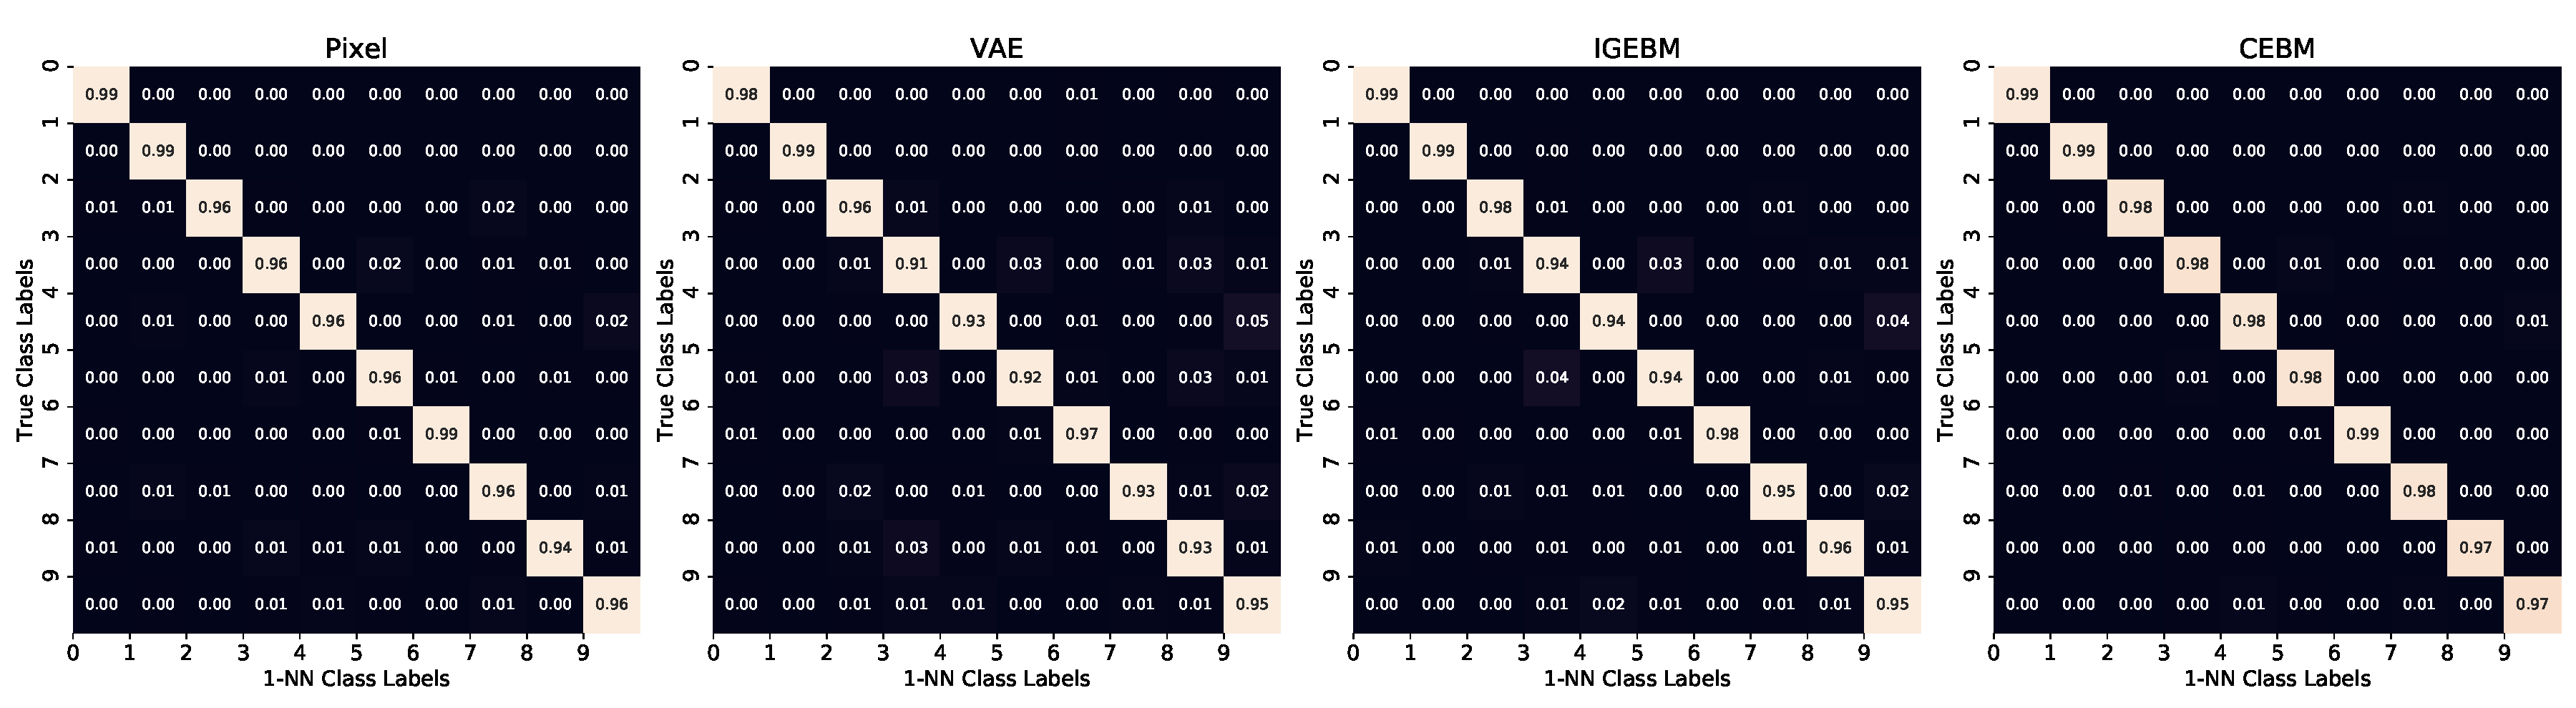
\includegraphics[width=\linewidth]{figures/confusion_matrix_14row_mnist.pdf}
\caption{MNIST}
\label{appendix:confusion-matrices-mnist}
\end{figure}
\begin{figure}[!h]
\centering
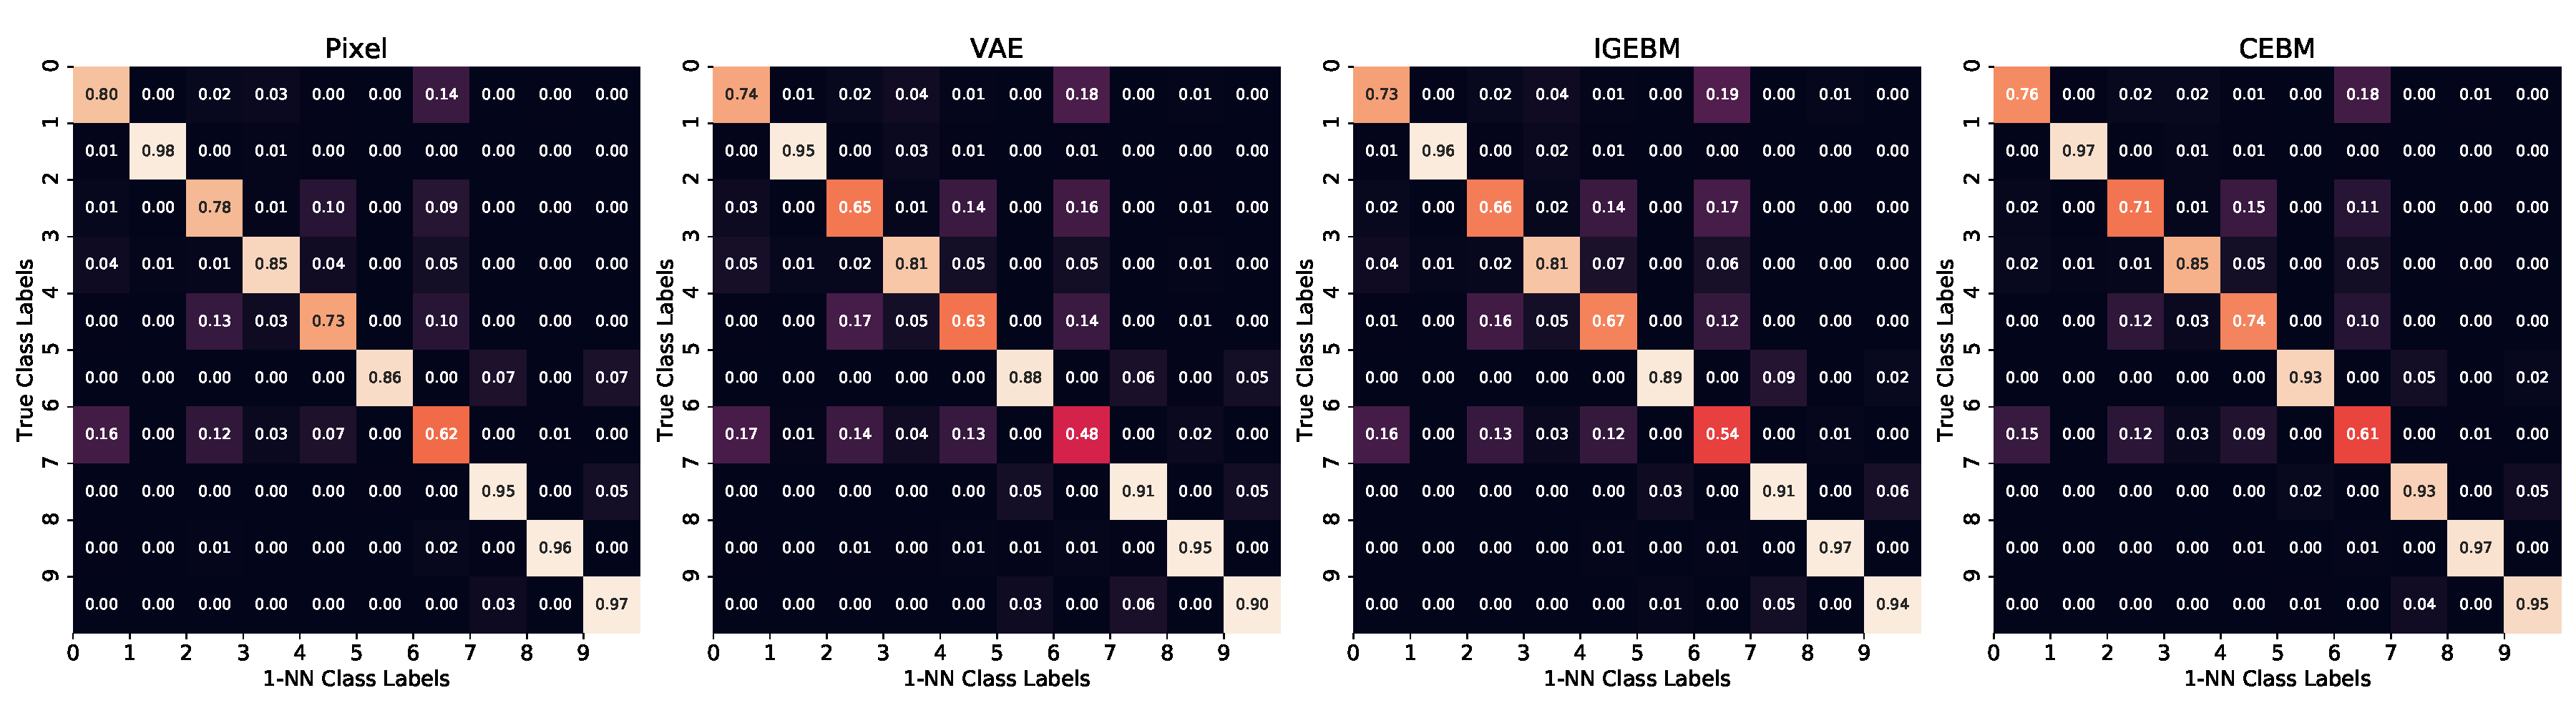
\includegraphics[width=\linewidth]{figures/confusion_matrix_14row_fashionmnist.pdf}
\caption{Fashion-MNIST}
\label{appendix:confusion-matrices-fmnist}
\end{figure}
\vspace{-2em}
\begin{figure}[!h]
\centering
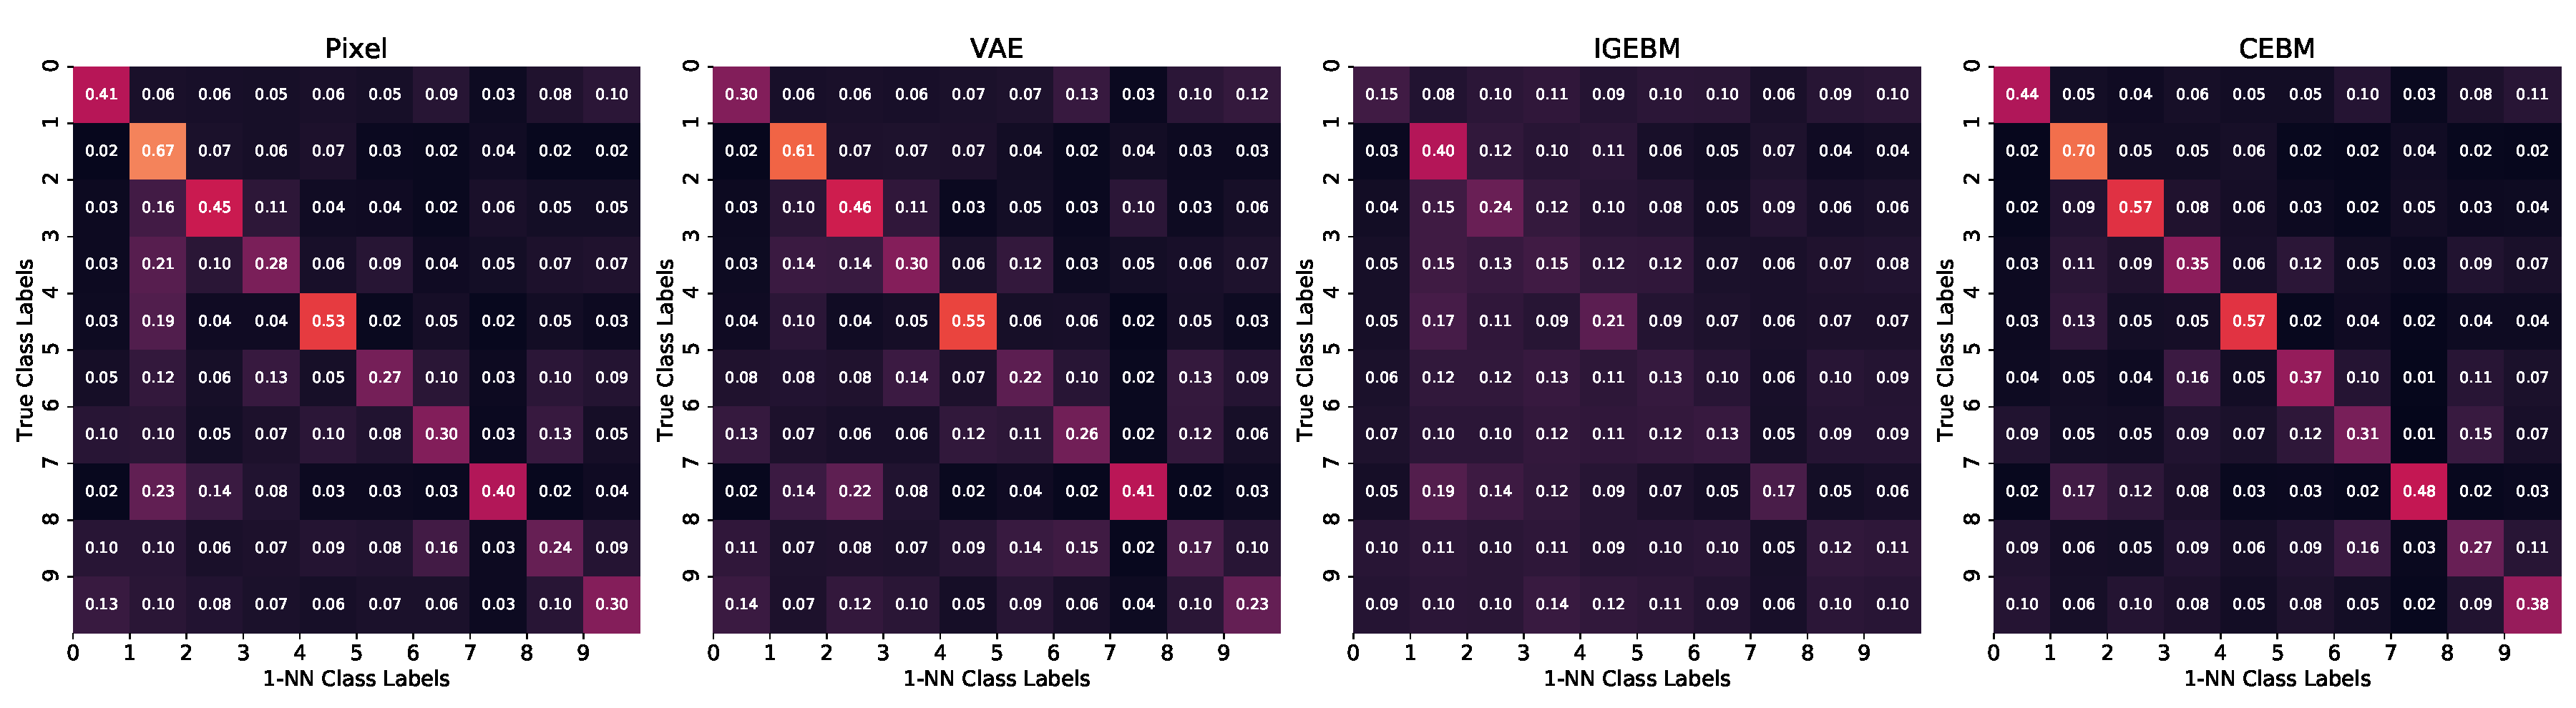
\includegraphics[width=\linewidth]{figures/confusion_matrix_14row_svhn.pdf}
\caption{SVHN}
\label{appendix:confusion-matrices-svhn}
\end{figure}
\vspace{-2em}
\begin{figure}[!h]
\centering
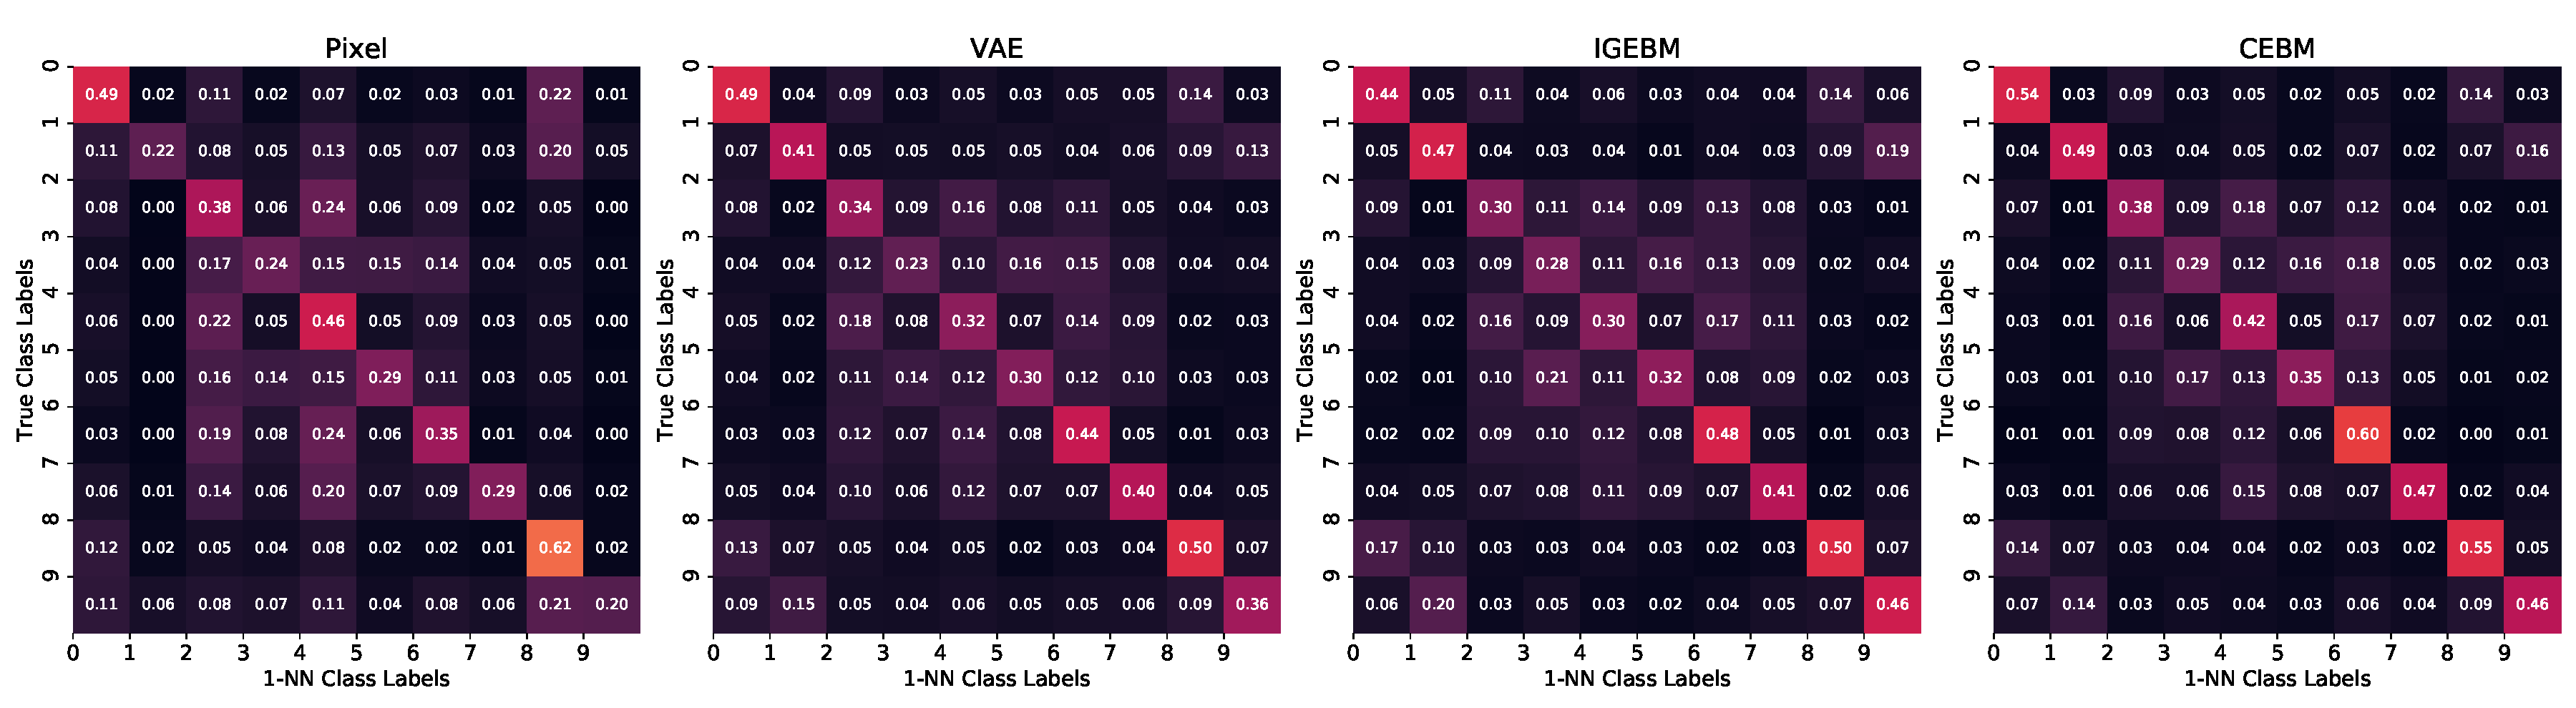
\includegraphics[width=\linewidth]{figures/confusion_matrix_14row_cifar10.pdf}
\caption{CIFAR10}
\label{appendix:confusion-matrices-cifar10}
\end{figure}

\newpage
\subsection{Out-of-Distribution Detection}
\label{appendix-sec:ood-detection}
We compute the AUROC score in OOD detection based on two different score functions.



% \setlength{\tabcolsep}{4.5pt}
% \begin{table*}[!h]
% \caption{AUROC scores in OOD Detection. We use $\log p_{\q}(\vx)$ and $\| \nabla_{\vx}\log p_{\q}(\vx)\|$ as score functions.The left block shows results of the models trained on F-MNIST and tested on MNIST, E-MNIST, Constant (C); The right block shows results of the models trained on CIFAR-10 and tested on SVHN, Texture and Constant (C).}
% \centering
% \begin{tabular}{l|ccc|ccc||ccc|ccc}
% \toprule
% & \multicolumn{6}{c||}{Fashion-MNIST} &    \multicolumn{6}{c}{CIFAR-10}\\
% & \multicolumn{3}{c|}{$\log p_{\q}(\vx)$} & \multicolumn{3}{c||}{$\| \nabla_{\vx}\log p_{\q}(\vx)\|$} &  \multicolumn{3}{c|}{$\log p_{\q}(\vx)$} & \multicolumn{3}{c}{$\| \nabla_{\vx}\log p_{\q}(\vx)\|$}\\
% \midrule
%             &  MNIST  & E-MNIST& C &  MNIST & E-MNIST & C &  SVHN & Texture & C &  SVHN & Texture & C \\
% \midrule
% VAE         & 50 & 39 & 9 & 61 & 57 & 1  & 42 & \textbf{58} & 41 & 38 & \textbf{51} & 37 \\
% IGEBM       & 35 & 36 & 90 & 78 & 82 & 96& 45 & 31 & 64 & 33 & 17 & \textbf{62} \\
% CEBM        & 37 & 34 & 90 & \textbf{82} & \textbf{89} & \textbf{98} & 47 & 32 & \textbf{66} & 31 & 17 & 54 \\
% CEBMM       & \textbf{56} & \textbf{56} & \textbf{92} & 56 & 80 & 95     & \textbf{55} & 30 & 62 & \textbf{40} & 23 & \textbf{62}  \\
% \bottomrule
% \end{tabular}
% \label{tab:ood-detection}
% \end{table*}

\begin{table}[!h]
    \centering
    \label{tab:ood-detection}
    \subtable[Models Trained on Fashion-MNIST.][c]{
    \begin{tabular}{l|ccc|ccc}
    \toprule
    % & \multicolumn{6}{c||}{Fashion-MNIST} \\
    & \multicolumn{3}{c|}{$\log p_{\q}(\vx)$} & \multicolumn{3}{c}{$\| \nabla_{\vx}\log p_{\q}(\vx)\|$} \\
    \midrule
    &  MNIST  & E-MNIST& C &  MNIST & E-MNIST & Constant  \\
    \midrule
    VAE         & 50 & 39 & 9 & 61 & 57 & 1   \\
    IGEBM       & 35 & 36 & 90 & 78 & 82 & 96 \\
    CEBM        & 37 & 34 & 90 & \textbf{82} & \textbf{89} & \textbf{98}  \\
    CEBMM       & \textbf{56} & \textbf{56} & \textbf{92} & 56 & 80 & 95      \\
    \bottomrule
    \end{tabular}
    }
    % \vspace{*1em}
    \subtable[Models Trained on CIFAR-10.][c]{%
    \label{}
    \begin{tabular}{l|ccc|ccc}
    \toprule
    & \multicolumn{3}{c|}{$\log p_{\q}(\vx)$} & \multicolumn{3}{c}{$\| \nabla_{\vx}\log p_{\q}(\vx)\|$} \\
    \midrule
    &  SVHN & Texture & Constant &  SVHN & Texture & Constant \\
    \midrule
    VAE & 42 &  \textbf{58} & 41 & 38 & \textbf{51} & 37 \\
    IGEBM & 45 & 31 & 64 & 33 & 17 & \textbf{62} \\
    CEBM & 47 & 32 & \textbf{66} & 31 & 17 & 54 \\
    CEBMM & \textbf{55} & 30 & 62 & \textbf{40} & 23 & \textbf{62} \\
    \bottomrule
    \end{tabular}
    }
\caption{AUROC scores in OOD Detection. We use $\log p_{\q}(\vx)$ and $\| \nabla_{\vx}\log p_{\q}(\vx)\|$ as score functions. block shows results of the models trained on F-MNIST and tested on MNIST, E-MNIST, Constant; The right block shows results of the models trained on CIFAR-10 and tested on SVHN, Texture and Constant (C).}
\end{table}

\vspace*{-1.0ex}
% \subsection{Out-of-Distribution Detection}\label{sec:exp:ood}
% \vspace*{-1.0ex}

% EBMs have formed the basis for encouraging results in out-of-distribution (OOD) detection~\cite{du2019implicit,grathwohl2019your}. While it is not our focus in this paper, OOD detection can serve as an additional benchmark that helps evaluate whether a learned model accurately characterizes the data distribution. In Appendix~\ref{appendix-sec:ood-detection}, we report results in terms of two metrics. The first is the area under the receiver-operator curve (AUROC) when thresholding the log marginal $\log p_\q(x)$.  The second is the gradient-based score function proposed by ~\citet{grathwohl2019your}. CEBMs results for OOD detection in most cases improve upon VAE and IGEBM baselines.



% \setlength{\tabcolsep}{5pt}
% \begin{table*}[!t]
% \scriptsize
% \centering
% \begin{tabular}{l|ccc|ccc||ccc|ccc}
% \toprule
% & \multicolumn{6}{c||}{Fashion-MNIST} &    \multicolumn{6}{c}{CIFAR-10}\\
% & \multicolumn{3}{c|}{$\log p_{\q}(\vx)$} & \multicolumn{3}{c||}{$\| \nabla_{\vx}\log p_{\q}(\vx)\|$} &  \multicolumn{3}{c|}{$\log p_{\q}(\vx)$} & \multicolumn{3}{c}{$\| \nabla_{\vx}\log p_{\q}(\vx)\|$}\\
% \midrule
%             &  MNIST  & E-MNIST& C &  MNIST & E-MNIST & C &  SVHN & Texture & C &  SVHN & Texture & C \\
% \midrule
% VAE         & 50 & 39 & 9 & 61 & 57 & 1  & 42 & \textbf{58} & 41 & 38 & \textbf{51} & 37 \\
% IGEBM       & 35 & 36 & 90 & 78 & 82 & 96& 45 & 31 & 64 & 33 & 17 & \textbf{62} \\
% CEBM        & 37 & 34 & 90 & \textbf{82} & \textbf{89} & \textbf{98} & 47 & 32 & \textbf{66} & 31 & 17 & 54 \\
% CEBMM       & \textbf{56} & \textbf{56} & \textbf{92} & 56 & 80 & 95     & \textbf{55} & 30 & 62 & \textbf{40} & 23 & \textbf{62}  \\
% \bottomrule
% \end{tabular}
% \label{tab:ood-detection}
% \caption{AUROC scores in OOD Detection. We use $\log p_{\q}(\vx)$ and $\| \nabla_{\vx}\log p_{\q}(\vx)\|$ as score functions.The left block shows results of the models trained on F-MNIST and tested on MNIST, E-MNIST, Constant (C); The right block shows results of the models trained on CIFAR-10 and tested on SVHN, Texture and Constant (C).}
% \end{table*}


\end{document}
